\documentclass{article}
\usepackage{natbib}
\usepackage{makeidx}
\usepackage{graphicx}
\usepackage{fancyhdr}
\usepackage{url}
\usepackage{amssymb}
\usepackage{amsmath}
\usepackage{manfnt}
\usepackage{color}
\usepackage{verbatim}
\usepackage{bm} 
\usepackage{sfmath}
\usepackage{hyperref}

\newcommand{\ggb}{\color{blue}}
\newcommand{\ggr}{\color{red}}
\newcommand{\gggr}{\color{green}}
\newcommand{\ggob}{$\color{orange} \bullet$}
\newcommand{\gggb}{$\color{Green} \bullet$}
\newcommand{\ggrb}{$\color{red} \bullet$}
          
\renewcommand{\familydefault}{cmss}

\definecolor{shade}{gray}{0.8}

\baselineskip20pt

\textwidth470pt
\textheight670pt
\oddsidemargin0pt
%\leftmargin0pt
\topmargin-35pt

\newcommand{\Fst}{F_{\mbox{\footnotesize ST}}}
\newcommand{\Fis}{F_{\mbox{\footnotesize IS}}}


\makeindex

\pagestyle{fancy}

\usepackage{Sweave}
\begin{document}
\Sconcordance{concordance:Geneland.tex:Geneland.Rnw:%
1 42 1 1 0 2335 1}


\bibliographystyle{plainnat}

\thispagestyle{empty}
\setlength{\arrayrulewidth}{3pt}
\phantom{m}

\vspace{3cm}\begin{center}
\begin{tabular}{l}
\hline
\\
{\Huge \sf Population genetic and morphometric data analysis }\\
{\Huge \sf using R and the {\sc Geneland} program }\\
\\
%{\huge \sf  Gilles Guillot, Filipe Santos, Arnaud Estoup}\\
{\huge \sf The Geneland development group}
\\
\hline
\end{tabular}
\end{center}

\vspace{3cm}


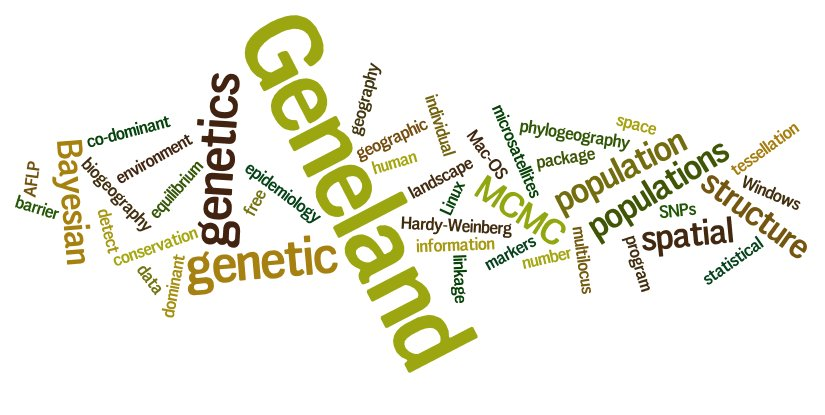
\includegraphics[height=8cm]{../inst/images/wdl1.jpeg}

\vspace{4cm}


\hspace{8cm} {\huge \em \today{}} \\


\setlength{\arrayrulewidth}{.5pt}
\newpage


%%%%%%%%%%%%%%%%%%%%%%%%%%%%%%%%%%%%%%%%%%%%%%%%

\tableofcontents

\newpage
%%%%%%%%%%%%%%%%%%%%%%%%%%%%%%%%%%%%%%%%%%%%%%%%


%%%%%%%%%%%%%%%%%%%%%%%%%%%%%%%%%%%%%%%%%%%%%%%%
\section{Overview}
\subsection{About {\sc Geneland}}

\subsubsection{How to request help}
If you are experiencing troubles with {\sc Geneland}, before requesting help, please 
\begin{itemize}
% \item make sure you are using the latest  versions of R and {\sc Geneland} (version numbers appear at loading)
\item read carefully the present documentation 
\item make sure you are able to describe and reproduce the problem you are experiencing
\end{itemize}

If you think you have identified a bug or feel the manual lacks information, you are welcome to report it. 
Then
\begin{itemize}

\item  send enough data and information about what you did in R  for us to reproduce the problem, namely
  \begin{itemize}
  \item on which operating system(s) did you experience trouble 
  \item if your problem is related to the use of {\sc Geneland} with the R command line, 
    give the exact sequence of commands that causes the problem
  \item  if your problem appears with the GUI, please generate and send the\texttt{ExecLog} file  
    located in the output directory (activate \texttt{Create Log file} option in top-left \texttt{Menu} panel.
  \item in any case, send a subset of your data that will allow us to reproduce the problem 
  \end{itemize}
\end{itemize}

Questions should be addressed to Gilles Guillot: \texttt{gilles.b.guillot[\`a]gmail.com}.


\subsubsection{History}
The work around {\sc Geneland} started in 2002-2003  at INRA in Avignon, France. 
This resulted in an algorithm to perform clustering under a spatial as well as a non-spatial model 
for codominant markers 
This algorihtm has been made available as a regular R package officially released on the Comprehensive R Archive Network in 2004. 
Filipe Santos joined the project in 2007 and wrote  the gra\-phical user interface in R-Tcl/Tk.
People who helped designing and improving the package includes:  
Arnaud Estoup, Annie Bouvier, Aur\'elie Coulon, Jean-Francois Cosson, Fr\'ed\'eric Mortier and Benjamin Guedj. 


Subsequent developments include a scheme accounting for the presence of null alleles \citep{Guillot08a}, 
an improvement of the  inference technique under the correlated frequency model \citep{Guillot08b}, 
a more efficient MCMC post-processing scheme \citep{Guillot08b}, 
an option to handle dominant markers \citep{Guillot10b}, 
a model to estimate the location and shape of hybrid zones \citep{Guedj11} 
and a generalisation of the model to deal with phenotype data \citep{Guillot12a}.
Axel Hille fulfilled a long-standing need of Geneland users by writing and sharing an R script showing how to 
combine {\sc Geneland} outputs with GIS data (section \ref{sec:AH}).

The program and its manual benefitted from comments from users registered on the {\sc Geneland} mailing list and also 
from discussions with people who attended courses  based on {\sc Geneland}. 
They are all warmly thanked.
 {\sc Geneland} is currently maintained by  Gilles Guillot. 

\subsubsection{Credit}
The {\sc Geneland} project received support from Institut National de le Recherche Agronomique, Bureau des Ressources G\'en\'etiques, 
Agence Nationale de la Recherche in France,  
the Norwegian Research Council, the Centre for Ecological and Evolutionnary Synthesis at the University of Oslo in Norway, 
the Technical University of Denmark in Copenhagen, the Danish Centre for Scientific Computing and the International Prevention Research Institute. 


%% \subsubsection{Contact, info, mailing list}\index{mailing list}\index{bug report}

%% %% {\sc Geneland} is distributed through the Comprehensive R Archive Network (CRAN). 
%% %% It consists of a network of mirroring sites throughout the world. 
%% %% This distribution method is very efficient but does not allow one to know how many users have downloaded or 
%% %% used a specific package.  
%% In order for people maintaining {\sc Geneland}  to have an idea about that 
%% and also for users to be informed of updates and related publications, 
%% a mailing list is operated. \\
%% Please register on \url{http://i-pri.org/special/Biostatistics/Software/Geneland/register.php}.


%% Reports of bugs in {\sc Geneland} and  errors  in the present manual are greatly appreciated.


\subsubsection{Citation}\index{citation}
Developing, improving and maintaining {\sc Geneland} represents a tremendous  amount of work.  
 If you use it for your own scientific work, 
please cite the related publications (\cite{Guillot05a},\cite{Guillot05c},\cite{Guillot08a},\cite{Guillot08b}, 
\cite{Guillot10b}, \cite{Guedj11}) 
detailed in the reference list at the end of the present document. 
For other references, type {\tt citation(``Geneland'')} in the R prompt or see the {\sc Geneland} homepage 
\url{i-pri.org/special/Biostatistics/Software/Geneland/} .



\subsection{System and hardware requirements}
\subsubsection{Operating system}

{\sc Geneland} is an add-on to the free statistical software {\sc R}. 
To install and run {\sc Geneland}, 
you need first to have R installed on your computer. R is available for MS-Windows, Linux and Mac-OS. \\
See \url{http://cran.r-project.org }.
See \url{ http://en.wikipedia.org/wiki/R\_(programming\_language)} for details.\\


 
\subsubsection{Memory}
Computations in {\sc Geneland} are carried out through a so-called Markov Chain Monte-Carlo (MCMC) technique. This implies that the 
overall computing task consists of a (very) long sequence of rather simple tasks. %% A small set of variables is stored in RAM, 
%% updated sequentially and written to the disk from time to time. This requires a few Mb  of RAM. The exact amount varies 
%% with datasets and computing options but it is fulfilled by any current computer. 
Since version 4.0.3, all MCMC output variables are stored in RAM during the MCMC computation and then stored after MCMC completion on the disk. 
This typically requires 50-500 Mb for standard datasets.

\subsubsection{Disk space}
The amount of disk space required depends on which fraction of the computations are stored on the disk. 
This amount can be fairly large from a few tens of Mega bytes to several Giga bytes 
(see section \ref{sec:faqthinning} for details). 

\subsubsection{Computer speed}
The model implemented in {\sc Geneland} is fairly complex. A  run of 100000 iterations for a dataset of 200 individuals at 10 loci) 
takes typically 3-15 minutes with a computer equipped with a 2 GHz chipset. This time depends on the 
model and storage options.

\subsection{Installation}

\subsubsection{Installing R}
Instructions for installation of R are continuously updated.\\
See \url{ http://cran.r-project.org/sources.html } for details and update.
 

Useful sources of information include the various R manuals \footnote{available from \url{http://cran.r-project.org}} and 
\citep{Paradis05,Paradis06} among others.
 
 
\subsubsection{Installing {\sc Geneland}}\label{sec:installGeneland}
 
As of version 4.9.0 (January 2020), Geneland is distributed via github.
See \href{https://github.com/gilles-guillot/Geneland}{https://github.com/gilles-guillot/Geneland} for installation instructions.

\subsection{Tasks performed}  
\subsubsection{Estimating the number of panmictic groups and locating their spatial boundaries}

The main task of {\sc Geneland} consists in clustering a sample 
into a certain number of groups in such a way that each group is homogeneous.
Since its earlier version, Geneland can process population genetics data, i.e. genotypes at several loci. 
For usch data, the main assumption is that the putative groups are 
approximately at Hardy-Weinberg equilibrium with 
linkage equilibrium between loci (HWLE). 

Since version 4.0.0, Geneland includes a model to deal with phenotypic data. 
See section \ref{sec:pheno} and \citet{Guillot12a} for detail. 

Different algorithms based on different models are implemented. The most popular algorithm is based on a spatial model 
and makes use not only of genotypes but also of spatial coordinates of sampled individuals (or populations). 

\subsubsection{Input files}



The research project that lead to the development of {\sc Geneland} was  focused on the combined use of genetics and geographic 
information to understand the factor affecting gene flow across space.
Hence, a typical dataset treated by {\sc Geneland} consists of 
\begin{itemize}
\item a file containing the genotypes of 
$n$ haploid\index{haploid} or diploid\index{diploid}  individuals at $L$ co-dominant  markers (micro-satellites, SNPs);
\index{micro-satellites}\index{SNP} 
\item a file containing the spatial coordinates representative of each individual.
\end{itemize}
This second file is actually optional and {\sc Geneland} can also be used without spatial information.
See section \ref{sec:data_format} for detail about data format.
As of version 4.0.0, Geneland can also process phenotypic data. 
The phenotypic data file should have one line per individual and one column per phenotypic variable. 

The program is able to deal with any combination of  phenotypic and genetic data, 
including situations where only phenotypic or only genetic data are available 
and situations when each individual is observed through its own combination of phenotypic and genetic markers. 
See Fig.~\ref{fig:global_dag} p.~\pageref{fig:global_dag} for an overview of the full model. 


\subsubsection{Output files and graphics}

The output of {\sc Geneland} consists of 
\begin{itemize}
\item an estimation of the number of HWLE populations, 
\item a map of the geographic spread of these various populations, 
\item a file giving  the estimated population membership of each individual
\item a file giving  the estimated population membership of pixel of the study domain (the size of the pixel 
being prescribed by the user).
\end{itemize}

Optional computing options allow to 
\begin{itemize}
\item account for null alleles (diploid data only)
\item account for spatial coordinates uncertainty
\end{itemize}

Additional outputs include
\begin{itemize}
\item computation of pairwise population $\Fst$
\item computation of individual population $\Fis$
\end{itemize}

%%%%%%%%%%%%%%%%%%%%%%%%
\section{Models}\label{sec:models}

Three types of quantities are involved:
\begin{itemize}
\item  the (usually unknown) number of populations $K$ 
\item the parameters (or hidden variable) coding for population membership (of individuals and pixels)
\item the parameters of the genetic model conditionally on the the number of populations and on 
population memberships.
 \end{itemize}

They are modelled separately. $K$ is assumed to follow a uniform distribution between 0 and 
an upper bound $K_{\max}$ 
prescribed by the user. The genetic and the spatial model are specified conditionally on $K$. 
This is described below. 



\subsection{Mixture models for genetic data}\label{sec:mixture}
\subsubsection{Diploid data: looking for within group Hardy-Weinberg and linkage equilibrium}

It is assumed that the overall dataset consists of individuals belonging to $K$ populations, 
each of these populations being 
at Hardy-Weinberg equilibrium with linkage equilibrium between loci. For $n$ individuals genotyped at $L$ loci, 
denoting by $f_{klj}$ the frequency of allele 
$j$ of locus $l$ in population $k$, by $p_i$ population membership of individual 
$i$ ($p_i  \in \{1,...,K\}$) and by 
$z_{il}=(\alpha_{il},\beta_{il})$ the genotype of individual $i$ at loci $l$, HWLE writes: 

\begin{equation}\label{eq:like}
\pi(z) = \pi((z_{il})_{il}) = \prod_{i=1}^n  \prod_{l=1}^L f_{p_il\alpha_i}f_{p_il\beta_i}(2-\delta_{\alpha_i}^{\beta_i})
\end{equation}

where $\delta_{\alpha_i}^{\beta_i}=1$ if $\alpha_i = \beta_i$  and  $0$ otherwise.


\subsubsection{Haploid data: multinomial distribution and linkage equilibrium}\index{haploid}
For haploid data, the model assumes a multinomial distribution of genotypes conditionally 
on allele frequencies and population memmberships and linkage equilibirum is also assumed.

\subsubsection{The uncorrelated frequency model}

Allele frequencies in the various sought populations are unknown and although they are not of direct interest, 
it is convenient to introduce them in the statistical computations. Indeed, once they are introduced and although 
they are unknown, Equation (\ref{eq:like}) allows to compute the  likelihood. Plugging this equation in an iterative scheme known 
as  Metropolis-Hastings algorithm\index{Metropolis-Hastings algorithm} allows to start from arbitrary values for  
all unknown parameters and to modify them in such 
a way that after many iterations, these values are close to the true values. 
The trick consisting in including extra unknown parameters in the inference not of direct interest but for 
computational purpose is known as data augmentation\index{data augmentation} in statistics. 


Once we have introduced the allele frequencies in the various sought populations, we need to place a prior distribution on them 
in view of Bayesian inference (see section~\ref{sec:algo}).

For each population and each locus, the entries of the vector $f_{kl1},...,f_{klJ_l}$ sum up to one. 
The simplest probability distribution fulfilling this condition is the Dirichlet distribution 
\footnote{See \url{ en.wikipedia.org/wiki/Dirichlet\_distribution}.}.
Beyond this algebraic property, 
it also has the interest to comply with a Wright-Fisher island model, the asymptotic distribution of allele frequency being 
Dirichlet under this model. 

This distribution depends on a single vector parameter which might vary across populations and loci. 
Assuming that this parameter $\alpha_{kl}$ is not common across 
populations and loci, assuming Dirichlet a priori distribution for $f_{klj}$ writes:
 \begin{equation}\label{eq:UFM}
\pi(f_{klj}) = \Gamma(J_l)
\end{equation}

This probability does not depend on the actual values taken by $f_{klj}$ and this model turns out to give the same 
a priori probability to any allele frequencies. 
The key assumption consists now in assuming that the vectors $f_{kl.}$ are mutually independent across populations. 
Independence  of the vectors $f_{kl.}$ is of course assumed across loci.


\subsubsection{The correlated frequency model}

The previous model is somehow over simplistic in the sense that most often, allele frequencies tend to be 
similar in different populations, 
(e.g. rare alleles  in a certain populations are also rare in other 
populations). From a statistical point of view, this property can be viewed as a correlation of $f_{klj}$ and $f_{k'lj}$ 
for some populations $k$ and $k'$.
This correlation can be viewed as a simple but useful summary of the common recent (micro-)evolutionary history of populations $k$ and $k'$.


The correlated frequencies model has been introduced previously 
(see e.g. \citep{Balding03},\citep{Nicholson02})  to account exactly for this property.


In this model, one introduces the frequencies of an ancestral population denoted by $f_{Alj}$ also assumed to be 
independently Dirichlet distributed and a vector of population specific drift parameters $(d_1,...,d_K)$ so that 
$f_{kl.}|f_A,d$ has a Dirichlet distribution
\begin{equation}
{ D}\left(f_{Al1}(1-d_k)/d_k,...,f_{AlJ_l} (1-d_k)/d_k\right)
\end{equation}
In this model and conditionally on $f_A$ and $d$, the frequencies are independent 
across populations, but marginally (integrating out $f_A$ and $d$) elementary computations (see \citep{Guillot08b}) 
show that the correlation of allele frequencies across population is:
\begin{equation}
% Cor(f_{klj},f_{k'lj}) = \frac{1}{1+ E[d_k]\frac{E[f_{Alj}]-E[f_{Alj}^2]}{E[f_{Alj}^2]-E[f_{Alj}]^2}}
Cor(f_{klj},f_{k'lj}) = 1\left/ \left[1+ E[d_k]\frac{E[f_{Alj}]-E[f_{Alj}^2]}{E[f_{Alj}^2]-E[f_{Alj}]^2}\right] \right.
\end{equation}
In the most general case, the distribution of the $f_{klj}$s in the uncorrelated model may depend on 
population-, locus- and allele-specific parameters 
$\alpha_{klj}$. In practice, the $\alpha_{klj}$ are always assumed to be common across  populations, locus and alleles,  and most often set to one. 
Similarly, in the correlated model, the $f_{Alj}$ might have locus- and allele-specific parameters but I do not consider this case here.
I set it to one as it is  most often done in practice, 
although the effect of this assumption has not been yet thoroughly assessed in the context of clustering 
(but see \citep{Foll08} in another context). 
Independence is always assumed across loci. 

Specifying fully the model also requires to place a prior on the drift parameters $d_k$. As this parameter 
has to lie in $[0,1]$, it is natural to 
consider a Beta prior, with independence across populations. A Beta distribution depends on two parameters. 


The correlated model can be viewed as a Bayesian 
and  biologically grounded way to make inference under the uncorrelated model with population-, locus- and allele-specific parameters. 


It has been observed that using the correlated frequency model could be more powerful at detecting subtle differentiations. 
On the other hand, 
this model seems to be more prone to algorithm instabilities and more sensitive to departure from model assumptions 
(e.g. presence of isolation-by-distance).  
It is recommended to start data analysis with the uncorrelated frequency model and then to check how these initial results 
are modified by the use of the correlated frequency model. It is also important to check ex-post that the inferred groups 
are significantly differentiated and at HWLE.


\subsection{Mixture model for phenotypic data}\label{sec:pheno}
We assume here  that we have a data-set consisting of  $n$ individuals sampled at sites ${\bf s}=(s_i)_{i=1,...,n}$ 
(where $s_i$ is the two-dimensional spatial coordinate of individual $i$),  
observed at some phenotypic variables denoted  ${\bf y}=(y_{ij})_{\substack{\;i=1,...,n \\j=1,...,q}}$.
 Our approach also encompasses the case where sampling locations are missing (or considered to be 
irrelevant). The only constraint that we impose is that if spatial coordinates are used, 
they must be available for all individuals.

As above, we assume that each  individual sampled belongs to one of $K$ putative clusters 
and that variation in the data 
can be captured by cluster-specific (location and scale) parameters. 


Denoting by $p_i$ the cluster membership of individual $i$ ($p_i \in \{1,...,K\}$), 
we assume that conditionally on $p_i=k$, $y_{ij}$ is drawn from a parametric distribution with cluster-specific parameters. 
Independence is assumed within and across clusters  conditionally on cluster membership. This means in particular that 
there is no residual dependence between variables not captured by cluster memberships. 
We assume  that the $y$ values arise from  a  normal distribution. 
Each cluster is  therefore characterized by a mean $\mu_{kj}$ and a variance $\sigma^2_{kj}$
and our model is a mixture of multivariate independent normal distributions. 
We use the natural conjugate prior family on 
 $(\mu_{kj},1/\sigma^2_{kj})$ for each cluster $k$ and variable $j$.
Namely, we  assume that the precision $1/\sigma^2_{kj}$ (i.e.  inverse variance)  follows  a Gamma distribution ${\cal G}(\alpha_{},\beta_{})$
($\alpha_{}$ shape, $\beta_{}$ rate parameter) and that conditionally on $\sigma_{kj}$, the mean $\mu_{kj} $ has a normal distribution  with 
mean $\xi_{}$ and variance $\sigma^2_{kj} / \kappa_{}$. 
In the specification above, $\alpha_{},\beta_{}, \xi_{}$ and $\kappa_{}$ are hyper-parameters. Details about their choice 
are  discussed in \citet{Guillot12a}. 


\clearpage
\subsection{Models underlying population membership}\label{sec:mbrship}


\subsubsection{The non-spatial model}
I denote by  $p$ a vector parameterising the  population memberships. 
In case population membership is modeled at the individual level, this vector can be simply $p=(c_1,...,c_n)$ 
where $c_i \in \{1,...,K\}$; In this case, the simplest form of prior that can be placed on it is an i.i.d prior $\pi(p|K) = 1/K^n$. 

Spatial representation for six simulations from this prior model are given on figure~\ref{fig:nonspaprior}.

\begin{figure}[h]
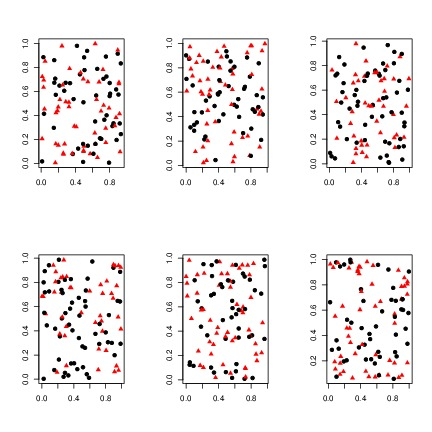
\includegraphics[height=12cm,width=17cm]{../inst/images/example_spatial_bis.jpeg}
\caption{Six examples of 100 individuals belonging to two populations spread totally at random across space.}\label{fig:nonspaprior}
\end{figure}

The previous model is numerically convenient but it is biologically questionable in the sense that one may wonder how differentiation 
might have occurred between populations in case of such spatial overlap between them.

\subsubsection{The spatial model}

This model consists in assuming that spatial domain of each population can be approximated by the union of a few polygonal domains, 
see figure~\ref{fig:spaprior} for examples. 

\begin{figure}[h]
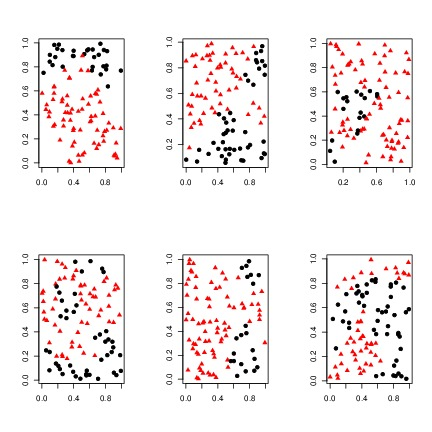
\includegraphics[height=12cm,width=17cm]{../inst/images/example_spatial2_bis.jpeg}
\caption{Six examples of 100 individuals belonging to two populations  where the 
spatial domain of each population can be approximated by the union of a few polygonal domains. }\label{fig:spaprior}
\end{figure}


This model corresponds to the spatial patterns that can be expected when differentiation occurs by limited gene flow induced by the presence 
of physical barriers such as road, rivers, mountain ranges, human activity.

Formally, the colored Poisson-Voronoi tessellation model consists in assuming that there is an unknown number of polygons $m$ 
that approximate the true pattern of population spread across space. 
These polygons are "centred" (this term is actually a bit inaccurate mathematically, but see below) around spatial points 
$u_1,...,u_m$ and each polygon belongs to one of the $K$ population which is coded by an integer (or color for graphical representation) 
denoted by $c_1,...,c_m$. Examples are given on figure~\ref{fig:spaprior2}. 


The exact mathematical definition of the colored Poisson-Voronoi tessellation model is as follows:
\begin{itemize}
\item the number of polygons follows a Poisson distribution with parameter $\lambda$: $m \sim \mbox{Poisson}(\lambda)$
\item conditionally on $m$, there are $m$ mutually independent points $u_1,...,u_m$ with uniform distribution over the study domain $D$:
$(u_1,...,u_m) |m \stackrel{\mbox{\footnotesize i.i.d}}{\sim} \mbox{Uniform}(D)$ 
\item each points $u_i$ defines a set $V_i$ of points in $D$ that are closer to $u_i$ than to any other points in $(u_1,...,u_m)$. 
This set $V_i$ is the i-th cell of the so-called Voronoi tessellation induced by $(u_1,...,u_m)$.
\item the points $(u_1,...,u_m)$ (or now equivalently the sets $V_1,...,V_m$) receive a mark with value in $\{1,...,K\}$ 
coding for population membership and displayed as different colors. These colors a assumed to be sampled from a probability distribution, 
which in {\sc Geneland} (but this is not a requirement) is assumed to be an independent, identically 
distributed and uniform distribution on $\{1,...,K\}$: 
$(c_1,...,c_m) |m \stackrel{\mbox{\footnotesize i.i.d}}{\sim} \mbox{Uniform}(\{1,...,K\})$ 
\end{itemize}

\begin{figure}[h]
\vspace{-1cm}
\begin{tabular}{cc}
\vspace{-1cm}
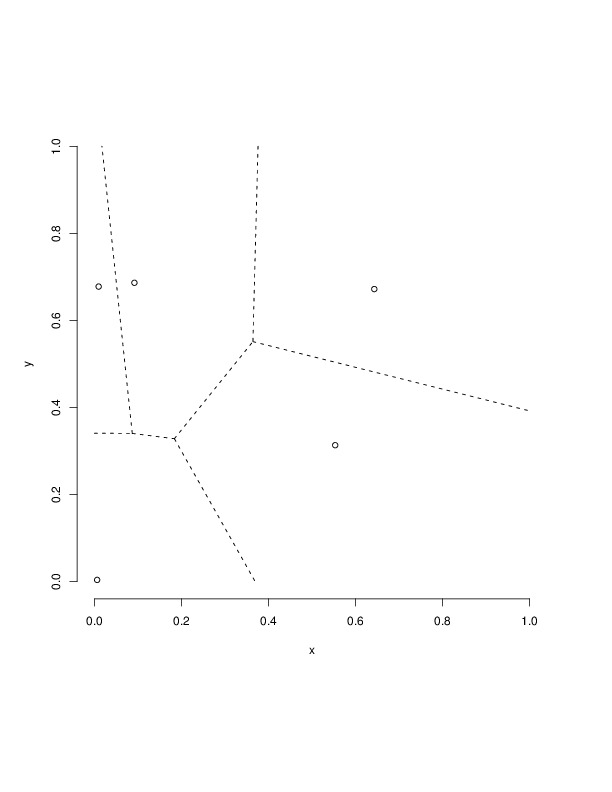
\includegraphics[height=10cm,width=7.5cm]{../inst/images/vor1.jpeg} & 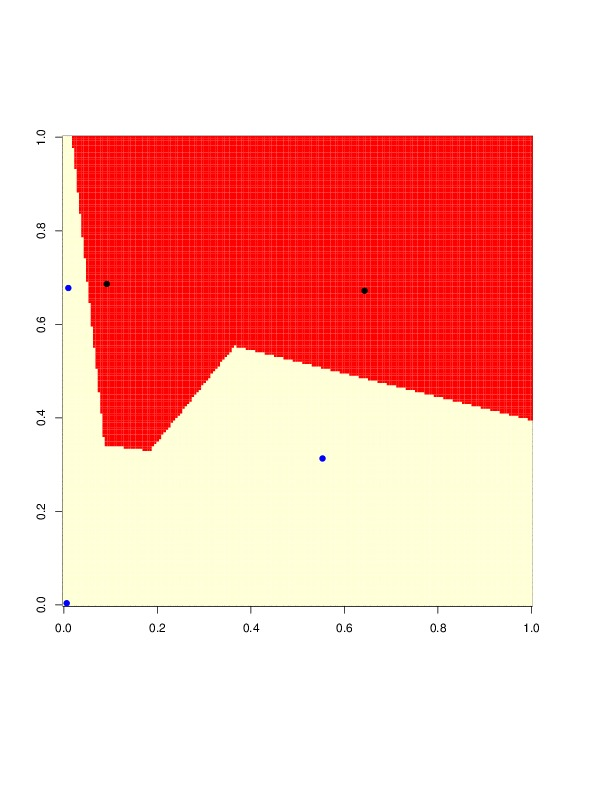
\includegraphics[height=10cm,width=7.5cm]{../inst/images/vor2.jpeg}
\end{tabular}
\caption{Example of colored Poisson-Voronoi tessellation. Left panel: location of cell "centre" and Voronoi cells induced. 
Right panel: a example of colored tessellation obtained after coloring at random each cell as red or white. 
In this example, the number of population $K=2$ and the number of polygons $m=5$.
There is no attempt to represent the location of any sampled individual.}\label{fig:vor}
\end{figure}

\begin{figure}[h]
\begin{tabular}{cc}
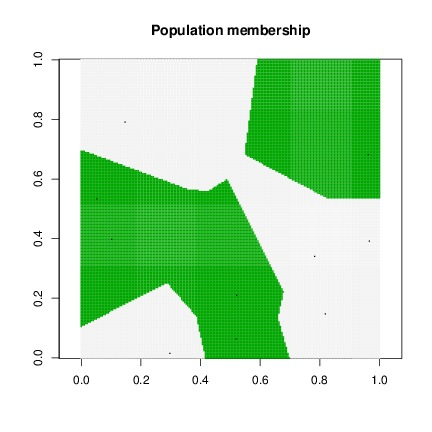
\includegraphics[height=9cm,width=8cm]{../inst/images/example_spatial3_bis.jpeg} & 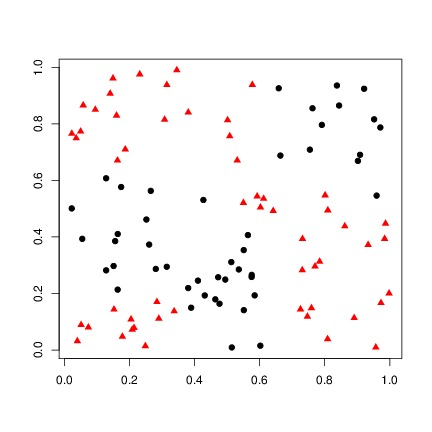
\includegraphics[height=9cm,width=7.6cm]{../inst/images/example_spatial3_ter.jpeg} \\
\end{tabular}
\caption{An example of 100 individuals belonging to two populations  where the 
spatial domain of each population can be approximated by the union of a few polygonal domains. Left: spatial spread of individuals, 
right: corresponding polygons. 
In this example, $n=100$, $K=2$ and the number of polygons $m=10$.
The points $u_i$ are depicted as tiny black dots on the left hand side panel. They are not depicted on the right hand side 
for clarity.}\label{fig:spaprior2}
\end{figure}



\subsection{Additional modelling options}

\subsubsection{Null alleles}\index{null alleles}\label{sec:null_alleles}

A well known source of potential problems is the
presence of null alleles arising from variation in the 
nucleotide sequences of flanking regions that prevent the primer annealing to template DNA during PCR amplification of 
the microsatellite locus \citep{Dakin04,Pompanon05}. 
The presence of null alleles results in an excess of homozygous genotypes within a population as compared to 
the expected proportion under Hardy Weinberg Equilibrium (HWE) and Linkage Equilibrium (LE)  \citep{Callen93,Paetkau95} while 
the model in {\sc Geneland} is based on HWE and LE within the sought clusters. 

In {\sc Geneland}, the putative presence of null allele(s) can be  explicitly taken into account for diploid data through an optional computing step. 
When this option is used, genotype ambiguity (homozigotes) is accounted for and null alleles frequencies is estimated 
along the clustering algorithm. 
With the option \texttt{filter.NA=TRUE} in function \texttt{MCMC}, 
null allele frequencies at each locus are estimated. 
They can be viewed with function \texttt{EstimateFreqNA}. 
This is also available through the GUI. 

Note that if this option is used in the default setting, 
all double missing genotypes will be interpreted as double
    null alleles. 
This can induce an over-estimation of null allele frequencies 
if some of the missing data are not null alleles 
(i.e. not due to amplification problems in the PCR), for example if some loci 
are missing for all individuals of certain sampling units. 
In order to minimize this kind of problems, an optional argument to function \texttt{MCMC} named \texttt{miss.loc} can be passed. 
The variable passed must be an $n \times L$  matrix (nb indiv. $\times$ nb loci). The entry of this matrix for line $i$ and column $l$ 
must be set to $1$ if there was no attempt to record the genotype of indiv. $i$ at locus $l$ ("genuine missing locus") 
and to $0$ otherwise (if data are available or are missing because  the PCR failed).
If no variable is passed to \texttt{miss.loc}, a matrix with only $0$s is passed by default and all double missing values 
will be treated as null alleles. 


\subsubsection{Coordinates uncertainty}\label{sec:uncertainty}\index{coordinates uncertainty}\index{uncertainty (on coordinates)}


You may want to treat the spatial coordinates as uncertain for any or a combination of the following reasons:
\begin{enumerate}
\item The individuals under study are non mobile (plants, animals species with very limited vagility as compared 
to the scale of the study domain) but the coordinates have been recorded with an error or they have been recorded 
with a limited precision only (e.g.  each individual has been affected to a small administrative unit).
\item The individuals under study are normally non mobile but a displacement might have been induced by the observation 
(e.g. hounding by hunters).
\item The individuals under study are mobile and they have a home range whose characteristic scale is non negligible 
as compared to the size of the study domain.
\item Even if none of the previous conditions  holds, but if your dataset has samples sharing the same coordinates, 
then allowing some uncertainty in the coordinates will allow to have samples with the same coordinates 
to be assigned to different populations. It can be useful to detect migrants. 
\end{enumerate}


Under conditions (1) and (2), the notion of "true" coordinates makes sense and refers to the location where each  
individual normally lives, but these locations have not been observed.
Under condition (3),  there is no "true coordinates", i.e. there is no particular location where each individual could 
be considered to live with certainty.
In  any of the previous conditions, the use of the recorded coordinates as locations where the individuals live
is inaccurate and can be misleading in the inferences.
It is recommended in this case to treat the observed coordinates as uncertain. The way {\sc Geneland} does it is to consider 
that the observed coordinate of each individual is the sum of the true coordinate and of a random noise of small magnitude. 
This random noise can be interpreted as the movement induced by capture in case of hounding (condition b), in the other cases 
it says that an individual has been observed somewhere but that it could have been observed anywhere around as well.

There is a parameter prescribing the amount of uncertainty attached to spatial coordinates (parameter \texttt{delta.coord} in function MCMC).

If this parameter is set to 0, spatial coordinates are
    considered as true coordinates, if this parameter is set to a value  \texttt{delta.coord}$>$0, 
it is assumed that observed
  coordinates are true coordinates blurred by an additive noise uniform
  on a square of side \texttt{delta.coord} centered on 0. It is assumed that this parameter is given in  the same units as 
the spatial coordinates. See also section \ref{sec:faq_uncertainty}. 




\begin{figure}[h]
\vspace{-2cm}
\hspace{-1cm}
\input{../inst/images/dag3.pdf_t}
\caption{Graph of the global model. 
Continuous black lines represent stochastic dependencies, dashed black lines represent 
deterministic dependencies. Boxes enclose data or fixed hyper-parameters, circles enclose inferred parameters. 
Bold symbols refer to vector parameters. 
The red, green and blue dashed lines enclose parameters relative to the phenotypic, 
geographic and genetic parts 
of the model respectively. The parameters of interest to biologists are the number of clusters $K$, 
the vector ${\bf p}$ which encode the cluster memberships,
and possibly  allele frequencies ${\bf f}$, mean phenotypic values $\bm{ \mu}$, phenotypic variance  $\bm{ \sigma^2}$ 
which quantify the genetic and phenotypic 
divergence between and within clusters. 
Other parameters can be viewed mostly as nuisance parameters.}\label{fig:global_dag}
\end{figure}

\clearpage


\subsection{Admixture model and hybrid zones}\index{admixture} \index{hybrid zone}

\subsubsection{Model}

In the models described in sections \ref{sec:mixture}-\ref{sec:mbrship}, each individual is assumed to have ancestries in one cluster only. 
This assumption might not be relevant, especially if the population under study undergone recent admixture events. 
Versions of {\sc Geneland} $\geq$  3.3.0 include a model where individuals have mixed ancestries \citep{Guedj11}. 
The likelihood of this model is similar to that of {\sc Structure} \citep{Pritchard00}.
Introducing the matrix $q=(q_{ik})$, where $q_{ik}$ refers to individual $i$'s genome proportion originating in cluster $k$, 
for diploid genotypes we have:
\begin{equation}\label{eq:admix_like}
L(z_{il} | f,q) = \sum_{k=1}^K q_{ik} f_{klz_{il1}}f_{klz_{il2}} (2- \delta_{z_{il1}}^{z_{il2}}) \;,
\end{equation}

and for haploid data we have

\begin{equation}\label{eq:admix_like}
L(z_{il} | f,q) = \sum_{k=1}^K q_{ik} f_{klz_{il}}\;.
\end{equation}
The model introduced now differs from earlier versions of {\sc Geneland} in that it  models admixture 
and from {\sc Structure} in that it is spatial. Those two features are accounted for as follows:
each vector of admixture proportions $q_{i.}=(q_{ik})_{k=1,...,K}$ is assumed to follow a  
Dirichlet distribution ${\cal D}(\alpha_{i1},...,\alpha_{iK})$.
We denote by $d_{ik}$ the distance of individual $i$ to cluster $k$ (in particular,  $d_{ik}=0$ 
if individual $i$ has been sampled in cluster $k$) 
and we assume a deterministic  relationship 
\begin{equation}\label{eq:def_alpha}
\alpha_{ik} = a\exp(-d_{ik}/b)
\end{equation}


By a standard property of the Dirichlet distribution, under equation (\ref{eq:def_alpha}) the expected value of $q_{ik}$ is 
\begin{equation}\label{eq:expect_q}
  E[q_{ik}] = \frac{e^{-d_{ik}/b}}{\sum_k e^{-d_{ik}/b}}
\end{equation}
In presence of $K=2$ clusters in contact along a hybrid zone, 
and if individual $i$ belongs to cluster $1$, 
then by definition $d_{i1}=0$ and we get 
\begin{eqnarray}
  E[q_{i1}] & = & \frac{e^{-d_{i1}/b}}{e^{-d_{i1}/b}+e^{-d_{i2}/b}} \nonumber \\
 & = & \frac{1}{1+e^{-d_{i2}/b}} \label{eq:expect_q_K=2}
\end{eqnarray}
i.e. the well known sigmoid function familiar to people studying hybrid zones.
Under this model, the width of the cline (defined as the inverse of the maximum gradient) is $w=4b$.
The variation of the expected admixture coefficients is illustrated in figure \ref{fig:exp_q}.


\begin{figure}[h]
\begin{tabular}{c}
\vspace{-.1cm}\hspace{3cm} 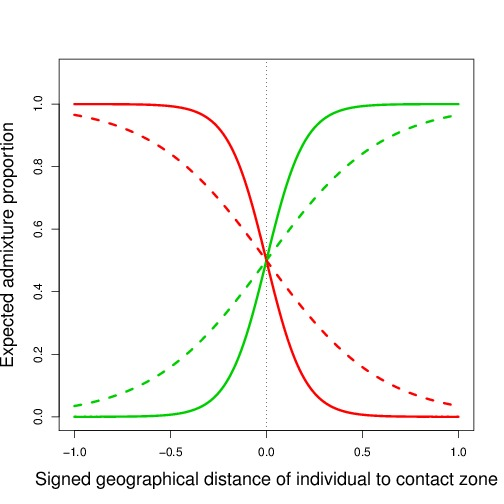
\includegraphics[width=9.5cm]{../inst/images/exp_q_quart.jpeg} \\
%\hspace{3cm} \includegraphics[width=9.5cm]{../inst/images/exp_q_vect.pdf}
\end{tabular}
\caption{Examples of spatial variation of expected admixture proportions in presence of two clusters. 
Individuals whose proportions are displayed here are assumed to be continuously located along a linear 
transect crossing perpendicularly a hybrid zone. 
 Red line: expected admixture proportion $q_{i1}$, 
green line: expected admixture proportion $q_{i2}$. 
Continuous lines: $a=1$, $b=0.1$, dashed lines: $a=1$, $b=0.3$.
Note that the curves are exactly sigmoid (logistic) functions. }\label{fig:exp_q}
\end{figure}

Parameter $a$ is a-dimensional, it does not affect the expected value of  $q_{ik}$ but 
controls its variance  with $V[q_{ik}] \propto 1/a$. 
Large $a$ values correspond to datasets with individuals displaying pretty similar admixture 
proportions within clusters.
Parameter $b$ is a spatial scale parameter, it has the dimension of a distance and is expressed in 
the same unit as spatial coordinates. 
Large $b$ values correspond to situations where admixture coefficients are loosely structured in space. 
At the limit where  $b= +\infty$, 
the vector $q_{i.}$ follows a flat Dirichlet distribution and the model does not display spatial features at all. 
Conversely, at the limit value $b=0$, all individuals display  admixture proportions that are 0 or 1 
with a spatial pattern mirroring exactly 
the underlying Poisson-Voronoi tessellation.
We place a uniform prior on $a$ and $b$ and assume independence of these two parameters.



%% \begin{figure}[h]
%% \begin{tabular}{c}
%% \vspace{-1.5cm}\hspace{3cm} \includegraphics[width=9.5cm]{../inst/images/exp_q_bis.pdf} \\
%% \hspace{3cm} \includegraphics[width=9.5cm]{../inst/images/exp_q_vect.pdf}
%% \end{tabular}
%% \caption{Examples of spatial variation of expected admixture proportions in presence of two clusters. 
%% Individuals whose proportions are displayed here are assumed to be continuously located along a linear 
%% transect crossing perpendicularly a hybrid zone. 
%%  Red line: expected admixture proportion $q_{i1}$, 
%% green line: expected admixture proportion $q_{i2}$. 
%% Top: the plots are obtained under sub-model (\ref{eq:def_alpha_c=1}).
%% Continuous lines: $a=1$, $b=0.1$, $c=1$, dashed lines: $a=1$, $b=0.3$, $c=1$, dotted lines:  $a=1$, $b=0.1$, $c=0.7$.
%% Note that for $c=1$ the curves are exactly logit functions. 
%% Bottom: the plots are obtained under model (\ref{eq:def_alpha}) with cluster-specific parameters. 
%% Continuous lines: $a_1=1$, $a_2=1$, $b_1=b_2=0.1$, $c_1=c_2=1$, 
%% dashed lines: $a_1=a_2=1$, $b_1=0.1$, $b_2=0.3$, $c_1=c_2=1$. 
%% }\label{fig:exp_q}
%% \end{figure}

\begin{figure}[h]
\centerline{\input{../inst/images/dag-final.pdf_t}}
\caption{Directed acyclic graph of the genetic model(s) implemented in {\sc Geneland}. 
Continuous lines represent stochastic dependencies, dashed lines represent 
deterministic dependencies. Squared boxes enclose data or fixed hyper-parameters, rounded boxes enclose inferred parameters. 
The thick green dotted line enclose parameters of the admixture model. }\label{fig:dag}
\end{figure}


\subsubsection{Inference  procedure}
An exact Bayesian inference would estimate all parameters of the admixture model 
by joint MCMC simulation of $(q,a,b)$ together with any other parameters involved in the model 
(number of gene pools, tessellation parameters and allele frequencies). 
We believe that the implementation of this strategy would offer a number of challenges, in particular when the number of clusters is unknown. 
For this reason, we suggest an alternative approximate two-stage strategy:

\begin{enumerate}
\item estimate allele frequencies and cluster locations under the non-admixture model. Denoting by $\theta_{\mbox{\tiny no adm.}}$ the vector of 
parameters in the no-admixture model, this amounts to sampling from $\pi(\theta_{\mbox{\tiny no adm.}} |z)$. This produces 
an estimate $\hat{\theta}_{\mbox{\tiny no adm.}}$, in particular it provides an estimate of the location of the putative hybrid zone. 
\item estimate  $(q,a,b)$ by MCMC simulation from the distribution of  $(q,a,b)$ conditionned by the data and the parameters estimates obtained from the non-admixture Geneland run. This amounts to sampling from  $\pi( (q,a,b) | \hat{\theta}_{\mbox{\tiny no adm.}} , z)$.
\end{enumerate}

With the command-line, the first step is implemented in function {\tt MCMC}, the second step in function {\tt HZ}.
Estimates of parameters of the hybrid zone model can be visualized with function {\tt show.estimate.hz}.
\clearpage
%%%%%%%%%%%%%%%%%%%%%%%%%%%%%%%%%%%%%%%%%%%%%%%%
\section{Data format}\label{sec:data_format}

\subsection{Genotypes file}\index{data format}


Assuming that you have data for $n$  individuals  genotyped at $L$ loci, 
the data must be arranged in 
\begin{itemize}
\item a plain ascii file 
\item without any extra invisible characters (like in MS-Word .doc files)
\item with one line per individual
\item each allele must be coded by an integer
\item the number of digits of each field is arbitrary and can vary across loci
\item extra header lines are not allowed when data are loaded via the GUI. 
Headers lines can be dealt with via the R function \texttt{read.table}. 
 The way these lines are handled when the data are loaded is prescribed 
through the arguments of \texttt{read.table}.\index{R function read.table}
\item missing data \index{missing data} are allowed. 
Users of the GUI have to specify the character string coding missing value in the \texttt{missing data symbol} sub-menu 
of the main menu. 
For users of the R command-line interface loading their data with the R function \texttt{read.table}, 
missing values can be coded in the raw text data file by any arbitrary character string, 
(e.g. {\tt000, 00, NA} or {\tt -999}). 
The character string used to encode missing data must be specified through the argument \texttt{na.strings} 
of function \texttt{read.table}. By default, when data are loaded through \texttt{read.table}, 
it is assumed that missing data 
are coded as {\tt NA}.
\item for haploid\index{haploid} organisms with $L$ loci, the genotype file must have $L$ columns.
\end{itemize}

\subsubsection{Diploid codominant data file}

This applies to microsatellites or SNPs data for diploid organisms.
The file should have one line and $2\times L$ columns per individual
For $L=10$, the two first lines of the genotype file should look like:\\

\medskip
\begin{verbatim}
198 000 358 3)62 141 141 179 000 208 224 243 243 278 284 86 88 120 124 238 244
200 202 000 358 141 141 183 183 218 224 237 243 276 278 88 88 120 124 240 244
.     .   .   .   .   .   .   .   .   .   .   .   .   .  .  .   .   .   .   .
.     .   .   .   .   .   .   .   .   .   .   .   .   .  .  .   .   .   .   .
.     .   .   .   .   .   .   .   .   .   .   .   .   .  .  .   .   .   .   .
\end{verbatim}

In the example above, missing values are coded as {\tt 000}. 
In the command line version, this file corresponds to argument {\tt geno.dip.codom} of function {\tt MCMC}.

\subsubsection{Diploid dominant data file}

This applies to AFLP data for diploid organisms.

The file should have one line and $L$ columns per individual. 
Absence or presence of the dominant allele should be coded as 0/1/ 
For $L=10$, the two first lines of the genotype file should look like:\\

\medskip
\begin{verbatim}
0 1 1 1 0 1 0) 0 0
1 0 0 1 1 0 0 1 000
. . . . . . . . .
. . . . . . . . .
. . . . . . . . .
\end{verbatim}

In the example above, missing values are coded as {\tt 000}.
In the command line version, this file corresponds to argument {\tt geno.dip.dom} of function {\tt MCMC}.

Diploid codominant data and diploid dominant data can be analyzed jointly.
Diploid dominant data and haploid data can not be analyzed jointly.

\subsubsection{Haploid data file}

This applies to microsatellites or SNPs data for haploid organisms or to mitochondrial DNA data. 

The file should have one line and $L$ columns per individual
For $L=10$, the two first lines of the genotype file should look like:\\

\medskip
\begin{verbatim}
198 000 358 3)62 141 141 179 000 208 224 
200 202 000 358 141 141 183 183 218 224 
.     .   .   .   .   .   .   .   .   . 
.     .   .   .   .   .   .   .   .   . 
.     .   .   .   .   .   .   .   .   . 
\end{verbatim}


In the example above, missing values are coded as {\tt 000}.
In the command line version, this file corresponds to argument {\tt geno.hap} of function {\tt MCMC}.

Diploid codominant data and haploid  data can be analyzed jointly.
Diploid dominant data and haploid data can not be analyzed jointly.

\subsection{Coordinates file}\index{data format}


\subsubsection{File format}

If you want to use the spatial model, you should  have a file containing spatial coordinates of the individuals sampled.
The coordinate  file must be such that  
\begin{itemize}
\item there is one line per individual and two columns (x-axis and y-axis coordinate), 
\item the units do not matter
\item it is assumed that the coordinates are planar coordinates such as 
UTM coordinates 
\item whether your coordinates are genuine planar coordinates or spherical coordinates does not 
appear in the file  format so that you can actually 
also input coordinates given as spherical coordinates. 
They will be interpreted as planar coordinates by 
the {\sc Geneland} functions. The quality of this approximation varies from very good (small domain, close to the equator) 
to very bad (large domain, close to a pole). 
\item extra header lines are not allowed when data are loaded via the GUI. 
Headers lines can be dealt with via the R function \texttt{read.table}. 
 The way these lines are handled when the data are loaded is prescribed 
through the arguments of \texttt{read.table}. \index{R function read.table}
\item missing data are not allowed in this file. 
\item if some coordinates are missing, you can either substitute an estimated value 
or do the analysis with {\sc Geneland} without spatial coordinates at all using the non spatial model. 
\end{itemize}


The two first lines  of a coordinate file should look like:\\



\medskip
\begin{verbatim}
25.6 745.2)
54.1 827.8
   .     .
   .     .
   .     .
   .     .
\end{verbatim}


%% \subsubsection{Pre-processing a coordinate file to convert spherical coordinates into planar projection coordinates}\index{Lambert coordinates}
%% \index{spherical coordinates}\index{longitude, latitude}

%% This can be done by the following steps:\\
%% \begin{verbatim}
%% ## load pa))ckages
%% require(mapproj)
%% require(maps)

%% ## read raw data
%% coord.lonlat <- read.table("pathtomydata/coord_lonlat.txt") 

%% ## check
%% plot(coord.lonlat,type="n",xlab="Lon",ylab="Lat",asp=1)
%% points(coord.lonlat,col=2)
%% map(resol=0,add=TRUE)

%% ## convert (Lon,Lat) coordinates into Lambert 
%% mapproj.res <- mapproject(x=coord.lonlat[,1],
%%                           y=coord.lonlat[,2],
%%                           projection="lambert",
%%                           param=c(min(coord.lonlat[,2]),max(coord.lonlat[,2])))

%% ## save planar coordinates as a two-column matrix
%% coord.lamb <- cbind(mapproj.res$x,mapproj.res$y)

%% ## save as a suitable ascii input file under the Geneland GUI
%% write.table(coord.lamb,file="pathtomydata/coord_lamb.txt")
%% \end{verbatim}


\subsubsection{Pre-processing coordinates to convert Lon/Lat into UTM}\index{UTM coordinates} \index{Lon/Lat coordinates}

This conversion can be done by function {\tt convUL} of the R package {\tt PBSmapping} or by function {\tt mapproject}  
of the R package {\tt mapproj}.
To use function {\tt convUL}, your matrix of coordinates must have two columns named  {\tt ``X''} and  
{\tt ``Y''}, a projection attriubute ({\tt ``LL''} or {\tt ``UTM''}) and a zone attribute (a number between 1 and 60). 
For example, if your coordinate matrix is named {\tt coord} and is in Lont/Lat format, it can be refromatted in UTM by:

\begin{verbatim}
colnames(coord) <- c("X","Y")
attr(coord, "projection") <- "LL"
attr(coord, "zone") <- NA 
coord.utm <- convUL(coord)
\end{verbatim}

See {\tt ? convUL} for detail.


\subsection{Phenotypes file}\index{data format}


Assuming that you have data for $n$  individuals recognized by $q$ quantitative 
phenotypic variables, the data must be arranged in 
\begin{itemize}
\item a plain ascii file 
\item without any extra invisible characters (like in MS-Word .doc files)
\item with one line per individual
\item with one column per  quantitative phenotypic variable
\item the number of digits of each field is arbitrary and can vary across lines and columns
\item extra header lines are not allowed when data are loaded via the GUI. 
Headers lines can be dealt with via the R function \texttt{read.table}. 
 The way these lines are handled when the data are loaded is prescribed 
through the arguments of .\index{R function read.table}
\item missing data \index{missing data} are allowed. 
Users of the GUI have to specify the character string coding missing value in the \texttt{missing data symbol} sub-menu 
of the main menu. 
For users of the R command-line interface loading their data with the R function \texttt{read.table}, 
missing values can be coded in the raw text data file by any arbitrary character string, 
(e.g. {\tt000, 00, NA} or {\tt -999}). 
The character string used to encode missing data must be specified through the argument \texttt{na.strings} 
of function \texttt{read.table}. By default, when data are loaded through \texttt{read.table}, 
it is assumed that missing data 
are coded as {\tt NA}.
\end{itemize}


\clearpage
%%%%%%%%%%%%%%%%%%%%%%%%%%%%%%%%%%%%%%%%%%%%%%%%
\section[Examples with the GUI]{Examples of data analysis using the graphical user interface (GUI)}

\subsection{Launching the GUI}

\begin{itemize}
\item launch R
\item load {\sc Geneland} by typing \texttt{library(Geneland)} in the R prompt
\item launch the {\sc Geneland} GUI by typing \texttt{Geneland.GUI()} in the R prompt.
\end{itemize}

This will open open a window as below:\\

\centerline{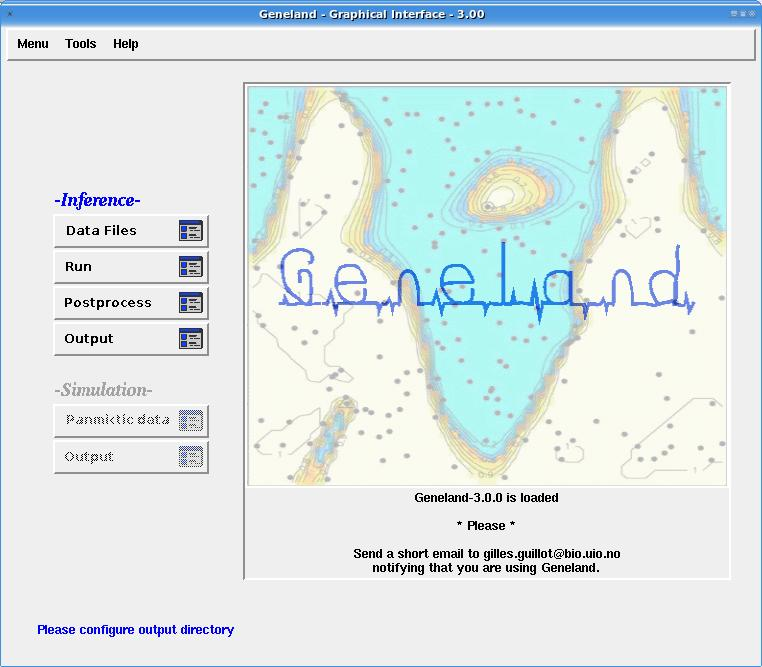
\includegraphics[width=11cm]{../inst/images/initial.jpg}}

\clearpage
\subsection{Selecting input and output files}


Select the fields separator in your data files:\\

\centerline{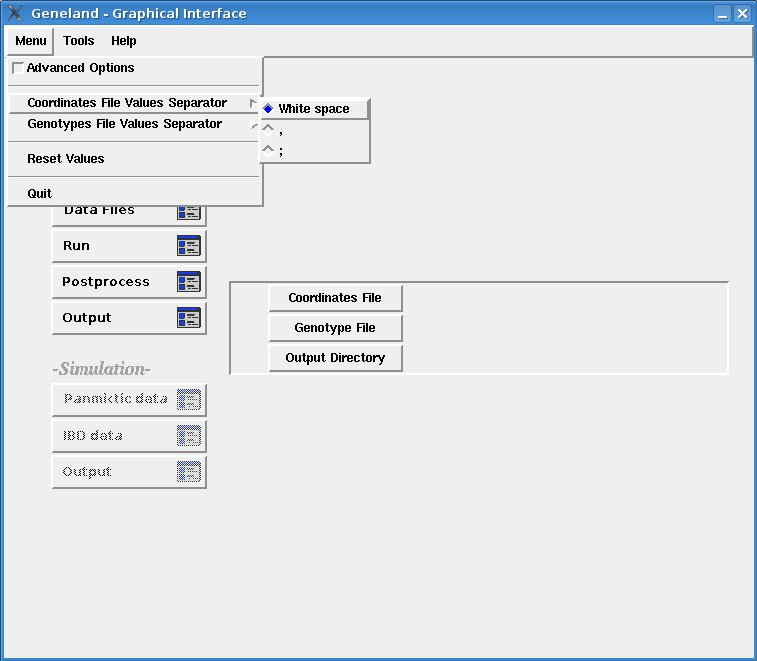
\includegraphics[width=11cm]{../inst/images/choosesep.jpg}}

\bigskip

Select  your data files and the directory containing your output files\\

\centerline{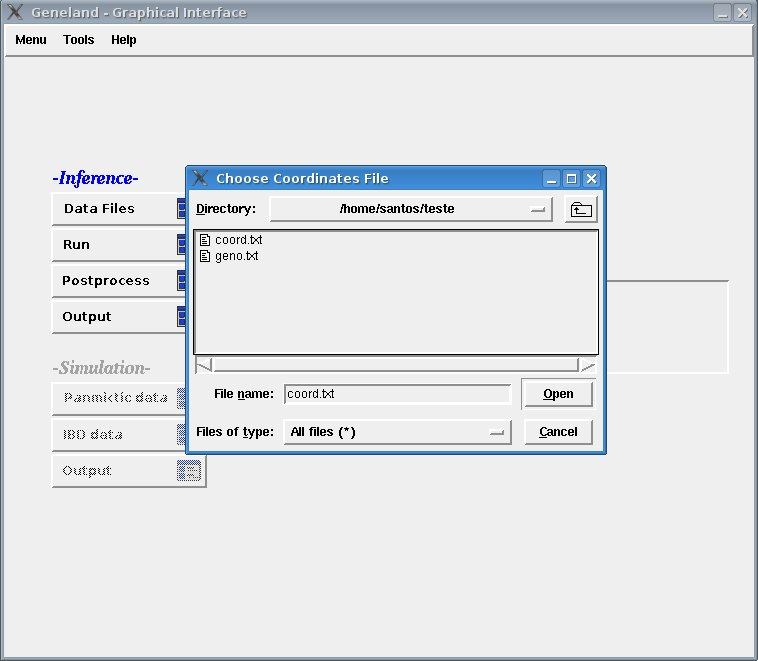
\includegraphics[width=11cm]{../inst/images/choosefiles.jpg}}


{\bf Important note:} the path can not be longer than 255 characters. 
You can avoid using long paths by selecting the working directory (under Windows) or by launching R in a  shell from 
a particular directory (under Linux). 

%\clearpage
\subsection{Inference}

We now carry out an analysis to infer the number of populations and their spatial boundaries for this dataset.
This can be performed by selecting MCMC simulation parameters as follows:\\

\centerline{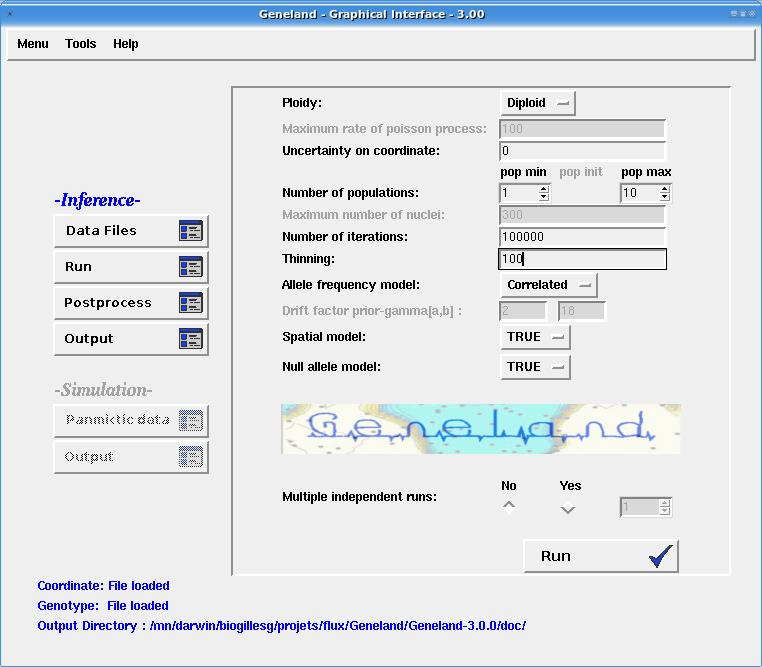
\includegraphics[width=11cm]{../inst/images/MCMC.jpg}}

\bigskip

In the above example we select

\begin{itemize}
\item diploid organism
\item no uncertainty attached to spatial coordinates
\item the number of HWLE populations is unknown and hence treated as simulated 
variable along the MCMC simulations allowed to vary between 1 and 10
\item the number of MCMC iterations will be $100000$ (\texttt{nit=100000}) 
\item and only each 100th iteration will be saved on the disk (in total, $1000$ iterations will be saved)
\item combined with 
the correlated frequency model (\texttt{freq.model="Correlated"}). 

\item using the spatial model (\texttt{spatial TRUE}), 


\item in the current working directory (\texttt{path.mcmc="./"}).
\end{itemize}


 

\clearpage
\subsection{Post-processing MCMC outputs}



The call to function \texttt{MCMC} generates different files in the directory specified by the argument \texttt{path.mcmc}. 
Information is extracted from this file through a call to function \texttt{Post.Process.Chain} as follows:\\


\centerline{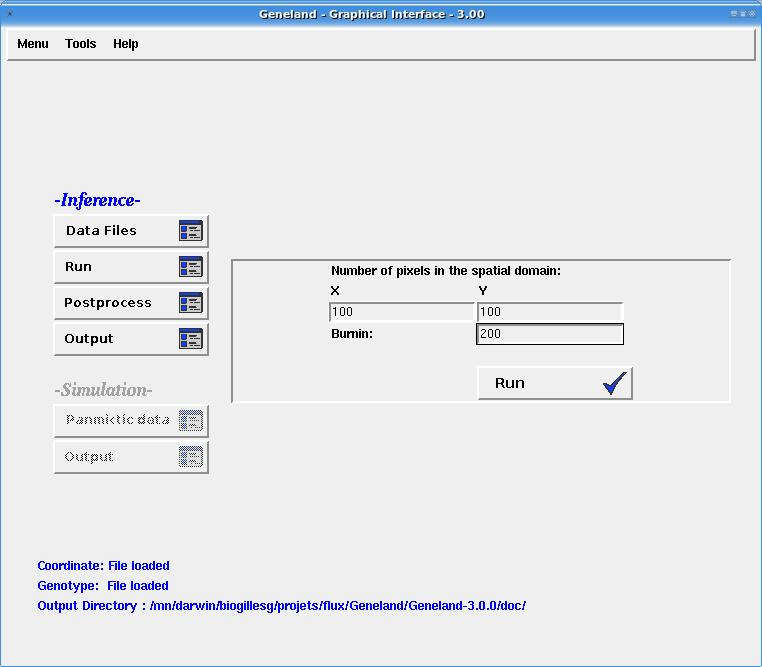
\includegraphics[width=11cm]{../inst/images/postproc.jpg}}

\bigskip

This will extract information from  MCMC simulation with 
\begin{itemize}
\item an horizontal  discretization of the study domain in 100 pixels (\texttt{nxdom=100})
\item a vertical  discretization of the study domain in 100 pixels (\texttt{nydom=100})
\item a burn-in of $200$ saved  iterations, i.e. discarding the $200$ first saved iterations (\texttt{burnin=200})
\end{itemize}
The parameters \texttt{nxdom} and \texttt{nydom} \index{nxdom,nydom} are only graphical parameters 
to set the resolution of the final maps. 


Here are some recomandations to set them.
\begin{itemize}
\item Set \texttt{nxdom} and \texttt{nydom} so as to avoid having two sampling sites in the same pixel.
\item Set \texttt{nxdom} and \texttt{nydom} so as to have the same resolution on both axis. For example, if you have 
a study domain of 300 km $\times$ 200 km, make sure that \texttt{nxdom} / \texttt{nydom} $\approx$ 3/2.
\item Avoid large values (larger than say 500). It would increase the resolution of the map in a way that is not visually detectable and it might saturate the virtual memory of your computer. 
\item The post-processing step is independent of the Markov chain computations and you can do as many tries as you want.. 
\item Why not having included the post-processing step as an automatic step of function MCMC? 
Because one may want to play with the burn-in and the resolution without re-launching the whole MCMC computations.
\end{itemize}


\clearpage
\subsection{Generating graphical and numerical outputs}

Clik on menu \texttt{output}:\\



\centerline{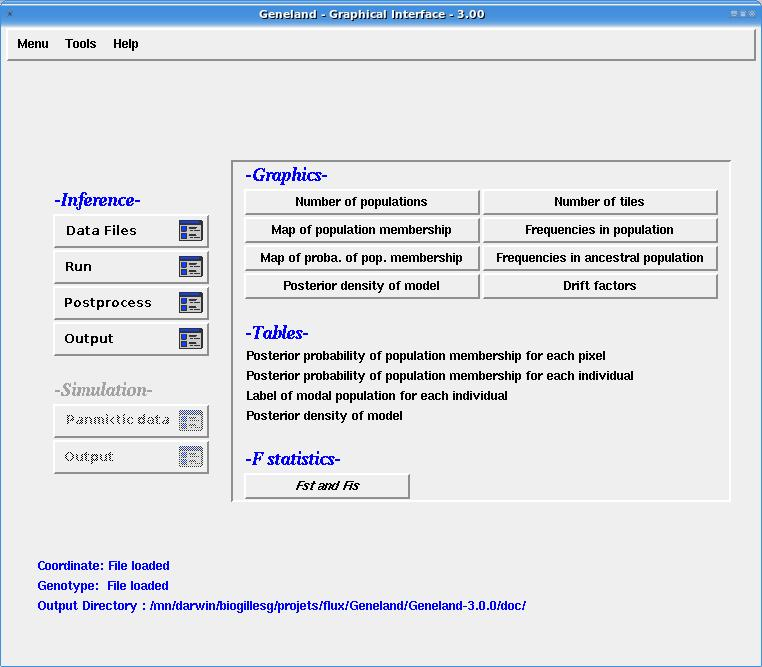
\includegraphics[width=11cm]{../inst/images/output.jpg}}

\bigskip

\clearpage
\subsubsection{Estimated number  of HWLE populations}
The number of population simulated from the posterior distribution can be visualised by clicking on \texttt{Number of populations}


This produces a plot like:\\

\centerline{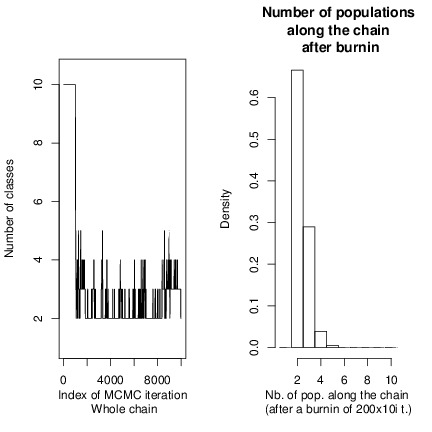
\includegraphics[height=10cm,width=11cm]{../inst/images/npop.jpeg}}

This run displays a clear mode at $K=2$ which is hence the {\em maximum a posteriori} estimate of $K$.\index{ maximum a posteriori}

\clearpage
\subsubsection{Map of estimated  population membership}
A map of estimated  population membership (by posterior mode) can be obtained by clicking \texttt{Map of population membership}


This produces a plot like:\\


\centerline{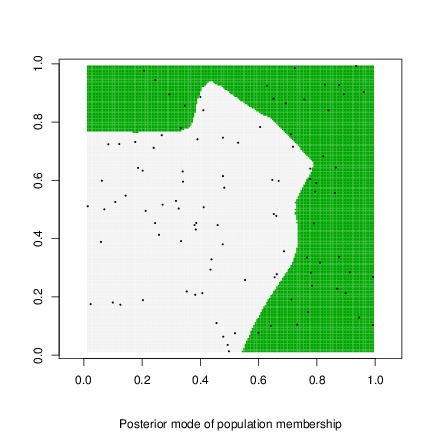
\includegraphics[width=12cm]{../inst/images/map.jpeg}}


\subsubsection{F statistics}
F statistics \cite{Weir84} relative to estimated clusters are obtained by:

\begin{verbatim}
Fstat.output(genotypes=geno,path.mcmc="./")
\end{verbatim}

which returns:

\begin{verbatim}
$Fis
[1] 0.1427044 0.1512689

$Fst
           [,1]       [,2]
[1,] 0.00000000 0.03562966
[2,] 0.03562966 0.00000000
\end{verbatim}


namely, individual  $\Fis$ and pairwise $\Fst$ for estimated clusters.

\clearpage
\subsection{MCMC inference under the admixture model}
 Assuming that you have an MCMC run under the non-admixture model, inference under the admixture model can be done as:
\begin{verbatim}
                 HZ(coordinates=coord,
                    geno.dip.codom=geno,
                    path.mcmc.noadm="path_to_noadmixture_mcmc_run/",
                    nit=20000,
                    thinning=10,
                    path.mcmc.adm="path_to_admixture_mcmc_run/")  

\end{verbatim}


In the below, the $a$ and $b$ parameters are fixed, the latest being large which corresponds to a situation of lose 
spatial structure of admixture coefficients. 
\begin{verbatim}
                 HZ(coordinates=coord,
                    geno.dip.codom=geno,
                    path.mcmc.noadm="path_to_noadmixture_mcmc_run/",
                    a.init=1,
                    b.init=1000,
                    a.max=10,
                    estimate.a=TRUE,
                    estimate.b=FALSE,
                    nit=20000,
                    thinning=10,
                    path.mcmc.adm="path_to_admixture_mcmc_run/")  

\end{verbatim}




\clearpage
\subsection{Launching several independent runs}

Inference is based on a stochastic method, i.e. for a given dataset, the values of estimated parameters are random and depend 
on what happened during the run. In theory, different runs should give approximately the same estimates provided they are long enough. 
A good way to check that a run was long enough is to launch different runs and check that they provide approximately the same parameter estimates 
($K$, individual population membership, maps).

This can be done automatically by clicking on the \texttt{Multiple independent runs} options:\\
\bigskip

\centerline{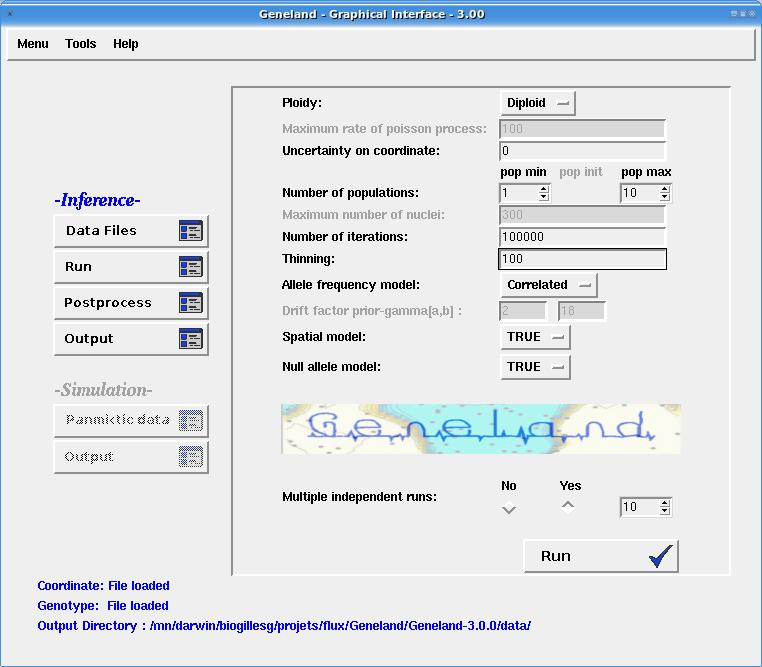
\includegraphics[width=12cm]{../inst/images/multip_run.jpg}}

\newpage
Runs are launched sequentially and computations are monitored in a new window:
\\
\bigskip

\centerline{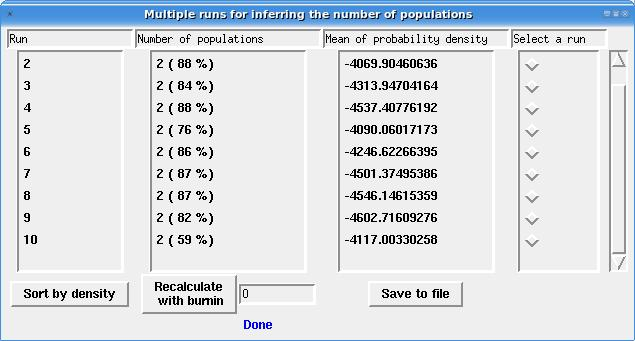
\includegraphics[width=12cm]{../inst/images/multip_run2.jpg}}


\bigskip

Here, the results of computations are consistent across runs in terms of estimated number of populations $K$. 
If different runs give different results, it is recommended to base conclusion on the run giving the highest average posterior 
probability (run $\#$ 2 above).

The MCMC output of these run is saved in the output directory. The output of each run is saved in a separate directory (named 1,2,...,).
The global ranking of the runs can also be saved in a file. 


\subsection{Parallel computations}

It is possible to take advantage of clusters and multi-core computers when running several independent runs. 
The supported parallelisation systems are MPI (Message Passing Interface) and PVM (Parallel Virtual Machine).

In order to use this feature you need to install the  R packages \texttt{snow} and \texttt{Rmpi} or \texttt{rpvm}.
This can be done for example via the  R command line by typing:
\texttt{install.packages("snow")}  and  
\texttt{install.packages("Rmpi")} 
or
\texttt{install.packages("rpvm")}.

Before starting the multiple runs go to the menu Tools and select the parallel processing. You should see a window like this:

\centerline{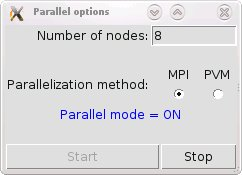
\includegraphics[width=4cm]{../inst/images/parallel.jpg}}

Here you choose the number of nodes ($>$ 1) and the parallelisation system (MPI or PVM). 
Then click start, when the message sets to ON then you can start your multiple run. 
Note that since inference is based on MCMC a  single run can not be run on several processors.

%%%%%%%%%%%%%%%%%%%%%%%%%%%%%%%%%%%%%%%%%%%%%%%%
\clearpage
\section[Examples with the command-line]{Example of data analysis using the R command-line}


  
\subsection{Preliminary steps}

\subsubsection{Organising your session}

If you plan to work through the R command-line, do not type directly the command in the prompt. 
Type them first in a data editor (the built-in command line editor under Windows or emacs under Linux). 
This allows you to keep a trace of your work not only as numerical output but also as something looking like 
a computer program that you can 
re-use, correct, modify, share later. In addition, storing R code often takes far less disk space than storing 
the numerical output.

\subsubsection{Launching {\sc Geneland}}
Assuming R and {\sc Geneland} are installed, 
\begin{itemize}
\item launch R
\item you can launch the on-line help by typing {\tt help.start()} in the R prompt (optional but very useful)
\item load {\sc Geneland} by typing {\tt library(Geneland)} in the R prompt
\item under Mac-OS, make sure that   X11 is launched (see section~\ref{sec:installGeneland}).\index{Mac-OS}
\end{itemize}

\subsubsection{Loading the data}


Let us assume that the data file(s) are named \texttt{genotypes.txt} and \texttt{coordinates.txt} 
and stored in a directory called \texttt{data}.
Then type in the R prompt:

\begin{verbatim}
geno <- read.table("../data/genotypes.txt",na.string="000") ## change "000" to according to your file
\end{verbatim}



... the genotypes are loaded and stored in an R object called \texttt{geno}.\\


Then type again in the R prompt:

\begin{verbatim}
coord <- read.table("../data/coordinates.txt")
\end{verbatim}



... the coordinates are loaded and stored in an R object called \texttt{coord}.\\


Generally you can replace {\tt ../data} by any string {\tt path\_to\_my\_data}  
giving the path  to the data relatively to the working directory. 
Under Windows this working directory is  specified through the menu file and sub-menu preferences. 
Under  Linux, the R working directory is the Linux working directory of the terminal  from which R was launched. 


\subsubsection{Checking the data}
You can control that you have correctly loaded your data by typing the names in the prompt, e.g.:

\begin{verbatim}
> coord[1:10,]
\end{verbatim}



will print the ten first lines of the coordinates.

The objects are a bit too large to be visualised in the R shell, it is more convenient to watch them through the built-in data editor:

\begin{verbatim}
fix(coord)
\end{verbatim}



or 

\begin{verbatim}
fix(geno)
\end{verbatim}



you can check the dimension of the object:

\begin{verbatim}
dim(coord)
\end{verbatim}



...we have indeed one line per individual and two columns, and...

\begin{verbatim}
nrow(geno)
\end{verbatim}



...one line per individual and ...\\

we have indeed one line per individual and two columns, and...

\begin{verbatim}
ncol(geno)
\end{verbatim}



two columns per locus for dipoloid data.\\


You can also plot the coordinates by 

\begin{verbatim}
plot(coord,xlab="Eastings",ylab="Northings",asp=1)
\end{verbatim}



...which opens a new window with the desired plot.


\subsection{Inference}\label{sec:example_MCMC}\index{MCMC}

We now carry out an analysis to infer the number of populations and their spatial boundaries for this dataset.
This is done with the main {\sc Geneland} function named {\tt MCMC}. 
A possible call of this function is as follows:

\begin{verbatim}
MCMC(coordinates=coord,
     geno.dip.codom=geno,
     varnpop=TRUE, 
     npopmax=10,
     spatial=TRUE,
     freq.model="Correlated",
     nit=100000,
     thinning=100,
     path.mcmc="./")
\end{verbatim}



This will perform parameter inference by MCMC simulation assuming 
that 
\begin{itemize}
\item the number of HWLE populations is unknown and hence treated as simulated 
variable along the MCMC simulations (\texttt{varnpop=TRUE}) 
\item but smaller than $10$ (\texttt{npopmax=10}), 
\item using the spatial model (\texttt{spatial=TRUE}), 
\item combined with 
the correlated frequency model (\texttt{freq.model="Correlated"}). 
\item the number of MCMC iterations will be $100000$ (\texttt{nit=100000}) 
\item and only each 100th iteration will be saved on the disk (in total, $1000$ iterations will be saved)
\item in the current working directory (\texttt{path.mcmc="./"}).
\end{itemize}


 
This function takes many more arguments, most of them being optionals (i.e. with default values).
An on-line help for function \texttt{MCMC} is given by typing \texttt{? MCMC}. See section \ref{sec:more_example}.


\subsection{Post-processing MCMC outputs}\index{PostProcessChain}

The call to function \texttt{MCMC} generates different files in the directory specified by the argument \texttt{path.mcmc}. 
Information is extracted from these files through a call to function \texttt{Post.Process.Chain} 
as follows:

\begin{verbatim}
PostProcessChain(coordinates=coord,
                 geno.dip.codom=geno,
                 path.mcmc="./",
                 nxdom=100,
                 nydom=100,
                 burnin=200)
\end{verbatim}



This will create additional files required to get final estimates and maps. In the example above, we have: 
\begin{itemize}
\item an horizontal  discretization of the study domain in 100 pixels (\texttt{nxdom=100})
\item a vertical  discretization of the study domain in 100 pixels (\texttt{nydom=100})
\item a burn-in of $200$ saved  iterations, i.e. discarding the $200$ first saved iterations (\texttt{burnin=200})
\end{itemize}


\subsection{Generating graphical and numerical outputs}

\subsubsection{Estimated number  of HWLE populations}
The number of population simulated from the posterior distribution can be visualised by:

\begin{verbatim}
Plotnpop(path.mcmc="./",
         burnin=200)
\end{verbatim}




This produces a plot like

\centerline{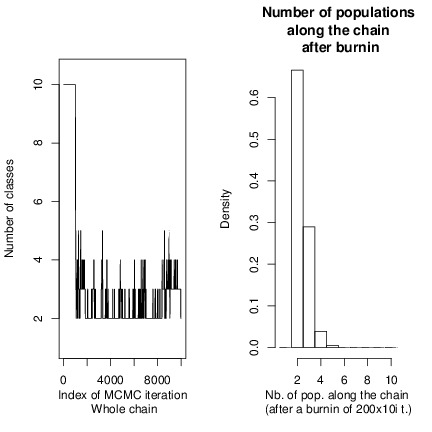
\includegraphics[height=10cm,width=11cm]{../inst/images/npop.jpeg}}

this run displays a clear mode at $K=2$ and a relatively good mixing around this value.


\subsubsection{Saving graphics}\index{postscript}\index{pdf}\index{graphical file format}

{\sc Geneland} functions for graphics contain arguments that allows users to send save graphics as pdf or postscript files. 
Here is an example:

\begin{verbatim}
Plotnpop(path.mcmc="./,
burnin=200,printit=TRUE,
file="Number_of_Clusters.pdf",format="pdf")
\end{verbatim}



\clearpage
\subsubsection{Map of posterior probability of population membership}

A call to function \texttt{PosterioMode} like:\\

\begin{verbatim}
PosteriorMode(coordinates=coord,
              path.mcmc="./",
              file="map.pdf")
\end{verbatim}




will produce a plot like:

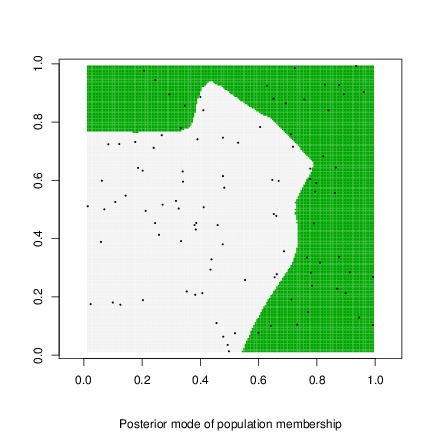
\includegraphics[width=12cm]{../inst/images/map.jpeg}

\subsubsection{F statistics}
F statistics relative to estimated clusters are obtained through

\begin{verbatim}
Fstat.output(genotypes=geno,path.mcmc="./")
\end{verbatim}



which returns:

\begin{verbatim}

$Fis
[1] 0.1427044 0.1512689

$Fst
           [,1]       [,2]
[1,] 0.00000000 0.03562966
[2,] 0.03562966 0.00000000
\end{verbatim}



namely, individual  $\Fis$ and pairwise $\Fst$ for estimated clusters.



\subsection{MCMC convergence assessment}


\subsubsection{Checking MCMC convergence, what does that mean?}

When it comes to Markov chains, convergence means that after enough iterations, the simulated vector is sampled from the 
desired target distribution. 
Since this target distribution is highly multi-dimensional and not much is known about it, checking convergence is not something easy to do 
and is actually most often impossible. 
The best that can be done is to check that there are no obvious clues indicating a lack of convergence. 
MCMC behaviours indicating a lack of convergence include:

\begin{itemize}
\item a single chain displaying a transient behaviour, for example a clear decreasing or increasing trend from its initial value 
\item multiple chains leading to different estimations (number of population $K$, population memberships)
\item a single chain stuck at a particular value or in a particular interval. Note however that in the case of a single integer parameters 
(for instance, the number of populations), a chain stuck at a particular value can be either a genuine feature of the posterior distribution 
or convergence flaw.
\end{itemize} 


See also an interesting page by Charlie Geyer advocating the use of a few long runs against many short runs:
\texttt{http://www.stat.umn.edu/\~{ }charlie/mcmc/one.html}.

\subsubsection{Factors affecting MCMC convergence}\label{sec:fact_MCMC_conv}

We have observed that mixing properties and hence convergence are affected by 

\begin{itemize}
\item the number of individuals $n$,  with poorer mixing properties as $n$ increases 
\item the number of loci $L$, with poorer mixing properties as $L$ increases 
\item departure from model assumptions. In case the dataset does not consist of genuine HWLE groups, it seems 
that the posterior distributions often exhibits  complex patterns of local modes in which MCMC simulations 
get more easily trapped. 
\end{itemize} 


\subsubsection{Example of R code as an aid to convergence diagnostic}
As explained above about the multiple runs option in the GUI, MCMC convergence should be checked by comparing the output of 
several independent runs. 

This can be done manually through a loop as follows:\\




\begin{verbatim}
## Loop for multiple runs
nrun <- 10
burnin <- 200
for(irun in 1:nrun)
  {
    ## define path to MCMC directory
    path.mcmc <- paste("./",irun,"/",sep="")   
    system(paste("mkdir ",path.mcmc))
    MCMC(coordinates=coord,
         geno.dip.codom=geno,
         varnpop=TRUE, 
         npopmax=10,
         spatial=TRUE,
         freq.model="Correlated",
         nit=100000,
         thinning=100,
         path.mcmc=path.mcmc)

    ## MCMC postprocessing
    PostProcessChain(coordinates=coord,
                     path.mcmc=path.mcmc,
                     nxdom=200,
                     nydom=200,
                     burnin=burnin)
  }
\end{verbatim}



\bigskip

\begin{verbatim}
## Computing average posterior probability
## with a burnin of 200 (* 100) iterations
lpd <- rep(NA,nrun)
for(irun in 1:nrun)
  {
    path.mcmc <- paste("./",irun,"/",sep="")
    path.lpd <- paste(path.mcmc,"log.posterior.density.txt",sep="")
    lpd[irun] <- mean(scan(path.lpd)[-(1:burnin)])
  }
\end{verbatim}



\bigskip

\begin{verbatim}
## Runs sorted by decreasing average posterior probability:
order(lpd,decreasing=TRUE)

\end{verbatim}




%%%%%%%%%%%%%%%%%%%%%%%%%%%%%%%%%%%%%%%%%%%%%%%%
\clearpage
\section[Influence of model assumptions]{Assessing influence of modelling assumptions}

\subsection{Choosing a model to perform MCMC simulations}

Computations are obtained under specific assumptions regarding allele frequencies (correlated/ non correlated) 
and population membership (spatial / non spatial). 
First you have to chose which combination of models is the most suitable for your data.
Roughly, if you expect differentiation due to the presence of simple shaped landscape features, the spatial model is presumably well suited. 
And if you are looking for low differentiation due to recent ecological events, the correlated allele frequencies model 
is more suitable. 

\subsection{Comparing outputs from MCMC runs under different models}

The estimates under your preferred model should be compared to estimates under other models. 
Note that even if a model is more realistic than others from the biological point of view, the results of analysis under this 
"best" model can be tricked by poor 
MCMC mixing. This can be    observed on large datasets ($> 1000$ individuals, $>100 loci$) and/or due to departure from modelling assumptions.


The most comfortable situation is when different models give similar answer. In this case, there is presumably a strong signal in the data 
and the inferred pattern does not depend on the particular way information is extracted (model+algorithm). \\
In case results differ across models, our recommendations are as follows:
\begin{itemize}
\item check convergence under the different models
\item give preference to models that fits better with the organism under study
  \begin{itemize}
  \item {\em a priori}: in the sense of prior knowledge about dispersal, potential barriers to gene flow...
  \item {\em a posteriori}: in the sense where estimated $K$ and maps complies best with what is known about the organism
  \end{itemize}
\item do not attempt to compare different models  on the basis of the average posterior probability. 
Indeed, they are defined on different parameter spaces and such a comparison do not make sense mathematically. 
\end{itemize}


\subsection{Objective criterions to perform model selection [TODO] }



%%%%%%%%%%%%%%%%%%%%%%%%%%%%%%%%%%%%%%%%%%%%%%%%
\clearpage
\section[Command line examples]{More examples using the R command-line}\label{sec:more_example}


\subsection[Null alleles]{Estimating frequency of null alleles}\index{null alleles}

If the option for filtering null alleles is chosen for simulation with function \texttt{MCMC}, the estimated frequency of null alleles at each locus 
can be obtained through function \texttt{EstimateFreqNA} as follows:

\begin{verbatim}
EstimateFreqNA(genotypes=geno,path.mcmc="./")
\end{verbatim}



which returns  a vector of length \texttt{nloc} (the number of loci) whose entries
  are estimated frequencies of null alleles.



\subsection[Non-spatial prior]{Analysing Geo-referenced data with a non-spatial prior}

A dataset consisting of Geo-referenced genetic data can be analysed with a non-spatial prior for population membership. 
The coordinates are not used in the inference algorithm, they are just used for the graphical representations. 

Similarly to the example of R code given in section \ref{sec:example_MCMC}, this can be done by:

\begin{verbatim}
MCMC(coordinates=coord,
     geno.dip.codom=geno,
     varnpop=TRUE, 
     npopmax=10,
     spatial=FALSE,          ## the argument spatial is now set to FALSE
     freq.model="Correlated"
     nit=100000,
     thinning=100,
     path.mcmc="./")
\end{verbatim}


\subsection{Analysing non spatial data}

It is also possible to analyse datasets consisting only of genotypes (no spatial coordinates). 
This can be done by  a call of function MCMC as:


\begin{verbatim}
MCMC(geno.dip.codom=geno, 
     varnpop=TRUE, 
     npopmax=10,
     spatial=FALSE,          ## the argument spatial set to FALSE
     freq.model="Correlated"
     nit=100000,
     thinning=100,
     path.mcmc="./")
\end{verbatim}



This allows to estimate the number HWLE populations and population memberships of individuals. 
Spatial graphical displays do not make sense in this context. 

\subsection{Getting improved graphics}
You may find that the graphical features available through the GUI and the {\sc Geneland} graphical functions are too limited. 
The possibilities to improve graphics by working directly though the command-line  are almost unlimited.



\subsection[Convergence checking]{Exploring MCMC outputs to better check convergence  [TODO]}



%\subsection{Interpretation of posterior probabilities of population memberships [TODO] }


\subsection[Displaying GIS data]{R and Geographical Information System (GIS) data}\index{GIS}

There exits many sites and specialised packages that you may find useful to handle your GIS data and combine them 
with {\sc Geneland} outputs. In this ection, we provide some pointers towards useful pages 
and try to a give a flavour of what is possible under R.


\subsubsection{Resources}

On the various formats and how to load them in R: \url{http://help.nceas.ucsb.edu/R:_Spatial}\\

Loading data, converting coordinates, plotting: \url{http://sites.google.com/site/spatialr}\\

Data (climate, landcover, coastal lines, administrative boundaries: \url{http://www.fao.org/geonetwork}\\


\subsubsection{Loading and plotting coastal lines}

An example with the FAO World Food Summit Map Coastline and International boundary (dataset available as a shapefile 
named wfs\_coas.shp from \url{http://www.fao.org/geonetwork}).

\medskip

\begin{verbatim}
library(maptools)
map <- readShapePoly("wfs_coas.shp")
plot(map,
     ## uncomment optionnal window limits
     # xlim=c(-5,15),ylim=c(40,60)
    )
\end{verbatim}


{\footnotesize  
\begin{verbatim}
library(maptools)
map <- readShapePoly("wfs_coas.shp")
plot(map,
     ## uncomment optionnal window limits
     # xlim=c(-5,15),ylim=c(40,60)
    )
\end{verbatim} }


\subsubsection{Superimposing countries boundaries and coast lines on a {\sc Geneland} map}

Let us assume that you have a map giving population memberships or posterior probabilities of population memberships over a given domain. 
You can superimpose countries boundaries and coast line by typing:

\begin{verbatim}
map(resolution=0,add=TRUE)
\end{verbatim}

 


This will add the desired lines to the active graphic window (by default the last window opened). 
The active graphic window can be redefined by e.g. \texttt{dev.set(3)} (this will set window \# 3 as active window). 
See on-line help of function \texttt{map} for details (\texttt{? map}).

\subsubsection{GRASS [TODO]}\index{GRASS}
Output of {\sc Geneland} can be combined with 
high quality maps obtained with the Geographic Resources Analysis Support System, commonly referred to as GRASS. 
See \texttt{http://grass.osgeo.org} and\\ \texttt{http://grass.osgeo.org/wiki/Main\_Page}.
Some of the tasks can be performed directly under R through the R package spgrass6.\\ 
See \texttt{cran.r-project.org/web/packages/spgrass6}.


\subsubsection[R plots and GoogleMaps]{Superimposing R plots on Google maps}\index{R package RgoogleMaps}

The R package {\tt RgoogleMaps} makes it possible to download Google maps, display and save them under R and superimpose 
other R grahical objects. This requires R package {\tt gdal} and libraries gdalconfig and proj\footnote{To be installed 
nder Ubuntu with sudo apt-get install gdalconfig proj. Not tested under Windows.}

Here is a small example. Assume you have a matrix of spatial coordinate named {\tt coord} looking like:\\

\begin{verbatim}
            > coord
            X        Y
            13.67137 55.60033
            13.62235 56.47770
            13.49812 55.95658
            17.44374 60.33607
            17.44306 60.32254
            16.08196 59.88587
            16.08384 60.11025
            20.98510 68.10043
            20.88659 67.65393
            22.17869 68.05858
            21.47275 67.63452
            20.43166 68.34153
            23.08695 67.11904
            22.51499 67.14419
            17.83787 63.15781
            17.76166 63.27629
\end{verbatim}



 
\medskip
Dowload the map:

\begin{verbatim}
MyMap.zoom8 <- GetMap(center=apply(coord[,2:1],2,mean), # center of area 
                                                        # (needs Lat/Lon 
                                                        # not Lon/Lat!)
                      zoom =8,  # resolution
                      maptype = "satellite")
\end{verbatim}


\medskip
To get a plot as in figure \ref{fig:Oslo_fjord}, type:

\begin{verbatim}
PlotOnStaticMap(MyMap.zoom8,
                lat=coord[,2] , lon= coord[,1] ,col='red')
\end{verbatim}


\medskip
Much more on the on-line help of R package {\tt RgoogleMaps} ({\tt ? RgoogleMaps}).

\begin{figure}[h]
\hspace{2cm}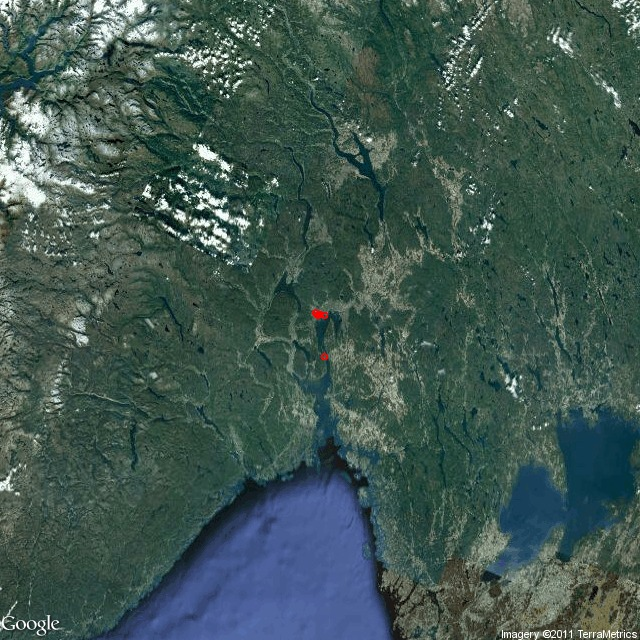
\includegraphics[width=5cm]{../inst/images/MyMap_zoom7.jpeg} \hspace{1cm}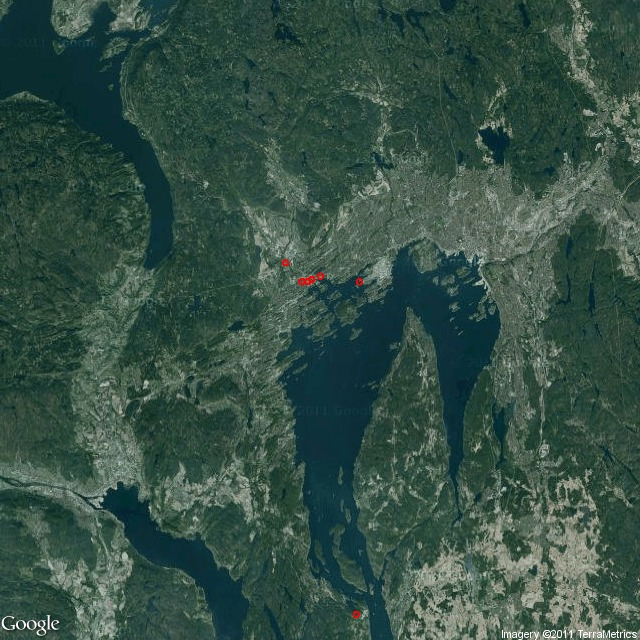
\includegraphics[width=5cm]{../inst/images/MyMap_zoom10.jpeg}
\caption{A rare sunny view of the Oslo fjord at two resolutions.}\label{fig:Oslo_fjord}
\end{figure}


\subsubsection[Displaying GIS data]{Displaying GIS data: A complete worked out example }\label{sec:AH}\index{GIS}

We  provide here a complete R script showing how Geneland outputs can be displayed using the various GIS 
R packages. This example is based on the book by \citet{Bivand08} and the case presented by \citet{Hille12}. 
The data used in this script are available from the Geneland homepage as 
\url{i-pri.org/special/Biostatistics/Software/Geneland/GIS_data} and \url{i-pri.org/special/Biostatistics/Software/Geneland/genetic_data}.
\index{R package rgdal}
\index{R package sp}
\index{R package maptools}
\index{R package shapefiles}
\index{R package tripack}

\verbatiminput{GGE_AH.R}
%\verbatiminput{test.R}
\clearpage


%%%%%%%%%%%%%%%%%%%%%%%%%%%%%%%%%%%%%%%%%%%%%%%%
\clearpage
\section{Simulation of data under the spatially organised HWLE populations model}\label{sim-HWLE}

Datasets can be simulated under the statistical models described in section \ref{sec:models}. 
This can be done via the R shell by calling function simFmodel as follows:

\begin{verbatim}
simdata <-  simFmodel(nindiv=100,
                      coord.lim=c(0,1,0,1),    ## simulations on the unit square
                      number.nuclei=15,        ## tessellation driven by 15 polygons
                      nall=rep(10,20),         ## 20 loci with 10 alleles each
                      npop=3,                  ## 3 populations
                      freq.model="Correlated", ## Correlated frequency model 
                      drift=rep(0.04,3),       ## drift (or Fst) parameters
                      dominance="Codominant"   ## codominant-like genotypes 
                      )                        ## (two columns per locus)
\end{verbatim}



Some of the arguments are optional. See on-line help (\texttt{? simFmodel}) for details.

The R object \texttt{simdata} is a list whose components can be checked by \texttt{summary(simdata)}. 
The genotypes are stored as \texttt{simdata\$genotypes} and the coordinates as \texttt{simdata\$coordinates} 
and are suitable for simulations studies, e.g. to assess the effect of number of loci, number of individuals, allele diversity ...
on accuracy of inferences. 


%%%%%%%%%%%%%%%%%%%%%%%%%%%%%%%%%%%%%%%%%%%%%%%%
\clearpage
\section[ Spatially correlated frequencies]{Simulation of data with spatially auto-correlated allele frequencies }\label{sim-IBD}\index{auto-correlated allele frequencies}

There is a function for simulation of data under the model described in \citep{Guillot09a}. 
This function is called {\tt simdata} and is an extension of function {\tt simFmodel} described in the previous section. It allows to simulate 
genotypes for individuals that are structured by isolation-by-distance and barriers to gene flow.
The function takes many arguments, most of them being optionnal. 
%% The complete list of arguments is as follows:
%% \begin{verbatim}
%% simdata(nindiv,
%%      coord.indiv ,
%%      coord.lim,
%%      rate ,
%%      number.nuclei ,
%%      coord.nuclei ,
%%      color.nuclei ,
%%      allele.numbers,
%%      IBD,
%%      model,
%%      alpha,
%%      beta,
%%      gamma,
%%      npop,
%%      seed.coord ,
%%      seed.tess ,
%%      seed.freq ,
%%      give.tess.grid=FALSE,
%%      give.freq.grid = FALSE,
%%      npix ,
%%      comp.Fst = FALSE,
%%      comp.Dsigma2=FALSE,
%%      comp.diff=FALSE,
%%      width,
%%      plot.pairs.borders=FALSE)
%% \end{verbatim}


See on-line help ({\tt ? simdata}) for detail about these arguments.

Here is an example for simulation of genotypes of 100 individuals at 3 loci with 5 alleles at each locus 
(values artificially small to limit the number of graphics generated in the next step). 

\begin{verbatim}
dataset <- simdata(nindiv=100,
                  number.nuclei=10,
                  allele.numbers=rep(5,3),
                  model="stable",
                  IBD=TRUE,
                  alpha=1,
                  beta=1,
                  gamma=1,
                  npop=3,
                  sim.gen=TRUE,
                  give.tess.grid=TRUE,
                  give.freq.grid=TRUE,
                  npix=c(100,100),
                  comp.Fst=TRUE,
                  comp.Dsigma2=TRUE,
                  comp.diff=TRUE,
                  width=0.1,
                  plot.pairs.borders=FALSE)
\end{verbatim}


The function returns a list stored in the R object {\tt dataset }.
Information about the object can be obtained by the function {\tt summary} as:

\begin{verbatim}
summary(dataset)
\end{verbatim}



The coordinates of individuals can be referred to by 

\begin{verbatim}
dataset$coord.indiv
\end{verbatim}



The genotypes of individuals can be referred to by 

\begin{verbatim}
dataset$genotypes
\end{verbatim}



The cluster membership of the individuals can be referred to by 

\begin{verbatim}
dataset$color.nuclei[dataset$nearest.nucleus.indiv]
\end{verbatim}





The simulated dataset can be visualised by function {\tt show.simdata} e.g. by

\begin{verbatim}
 show.simdata(dataset,
     plot.coord = TRUE,
     plot.tess = TRUE,
     plot.freq.grid = TRUE,
     loc.grid = 1,
     zlim.freq=c(0,1))
\end{verbatim}



 This will produce a plot of the coordinates of individuals, a map of the tessellation induced by the barriers simulated and 
maps of allele frequencies for alleles at the first locus ({\tt loc.grid=1}). 
See on-line help ({\tt ? show.simdata}) for details.

\clearpage
%%%%%%%%%%%%%%%%%%%%%%%%
\section{Using other softwares to analyse {\sc Geneland} outputs}

\subsection{Population genetics softwares}

\subsubsection{Genepop}
\index{Genepop}
There is a {\sc Geneland} function called \texttt{gl2gp} that writes coordinates and genotypes into an ascii file suitable for analysis 
with the \textsc{Genepop} program \citep{Rousset07}. See on-line help (\texttt{? gl2gp}) for details. 
The genotype file produced might require some extra hand editing.

\subsection{MCMC post-processing  softwares}
\subsubsection{Partitionview}
\index{Partitionview}

TODO
%% \texttt{Partittionview} can be used to visualise the posterior probability distribution of the partition of individuals. 
%% The information required as input for this program is in the file \texttt{proba.pop.membership.indiv.txt} stored in the {\sc Geneland} output directory. 
%% See section \ref{sec:proba.pop.membership.indiv.txt}. 

\subsubsection{Distruct}
\index{Distruct}
\texttt{Distruct} can be used to visualise the distribution of individual population membership. 
The information required as input for this program is in the file \texttt{proba.pop.membership.indiv.txt} stored in the {\sc Geneland} output directory. 
See section \ref{sec:proba.pop.membership.indiv.txt}. 
The information displayed is somehow similar to what is obtained with the {\sc Geneland} function \texttt{PlotTessellation} 
though disregarding the spatial aspect of the dataset. 

% \subsubsection{Clump}
% \index{Clumpp}
% \texttt{Clumpp} can be used relabel 



% \section{Analyzing other software's outputs [TODO]}

\appendix
%%%%%%%%%%%%%%%%%%%%%%%%
%%%%%%%%%%%%%%%%%%%%%%%%%%%%%%%%%%%%%
\clearpage
\section{Frequently asked questions}

\subsection{Can you provide sample input files?}\index{sample input files}
There are to be found in the directory {\tt data} of the Geneland distribution archive file.

\subsection{Can I use population data?}\index{population data}
It is possible to analyse datasets where different individuals share the same spatial location. 
If such data are treated without {\em uncertainty on coordinate } in the GUI or {\tt delta.coord} is set to 0 in function {\tt MCMC} 
then individuals sharing the same coordinates will be assigned to the same inferred group. 

\subsection{Can I use SNPs?}\label{sec:faq_SNPSs} \index{SNP}
It is possible to run {\sc Geneland} with SNPs. The bases have to be recoded as $\{1,2,3,4\}$.
Fixed alleles are not allowed. Loci carrying such alleles have to be removed from 
the dataset first. 

\subsection[Large number of loci]{How to deal with datasets containing a large number of loci?}
\subsubsection{Running {\sc Geneland} on a random subsets of loci}
You can run {\sc Geneland} for various random subsets of loci with e.g. 500-1000 loci and check that 
the different subsets give you the same answer. 
If this happens, you can confidently infer that runs with a larger number of SNPs would also give you the same answer. 
If different subsets give different answers, it can be due either to convergence issues (the genuine pattern contained in 
the various subsets is the same but {\sc Geneland} failed to detect it because of numerical difficulties) or 
to an excess of sampling variance in the selection of loci at random. There is no obvious way 
to decipher the relative importance of those two factors. 


\subsubsection{Managing output files}
By default, the Markov chain of all parameters are saved on the disk. The biggest files are usually those containing estimated allele 
frequencies (\texttt{frequencies.txt} and \texttt{ancestral.frequencies.txt}) and coordinates of nuclei of the Voronoi Tessellation 
(\texttt{coord.nuclei.txt}). It is recommended to compress or erase them after relevant information has been extracted from 
the corresponding runs. This requires to write a bit of R code  (see e.g. {\tt ? file.remove} or {\tt ? file}).

Multiples runs via the GUI should be avoided as it will quickly generate huge files.


\subsection{Can I use haploid data?}\index{haploid}
Yes. Specific computing options are implemented in {\sc Geneland} for haploid data. 

\subsection[Unusual ploidies]{Can I study organisms with ploidy other than haploid or diploid?}\index{ploidy $>$ 2}
No. The only ploidy handled as of today are haploid and diploid. 

\subsection{Can I use dominant markers?}\index{dominant markers}
Yes. 

\subsection[Special landscape features]{Is there any way to account for the presence of special landscape features?}
We have been often asked how to include information about the presence of "an urban area not suitable for my organisms" 
or "a land mass in the middle of sea water obviously not suitable for fish". 
There is currently no obvious way to do that with {\sc Geneland}. 
We recommend to analyse your data ignoring the presence of such landscape feature and to  try to take it into account 
at the post-processing stage. 

\subsection[Linear habitat]{Can I study an organism leaving in a linear habitat?}
Yes. The neat way to do that in {\sc Geneland} is to convert 2-dimensional coordinates into 1-dimensional curvilinear coordinates measuring distance 
of each individuals to an arbitrary origin in this habitat.

\subsection[MCMC jargon]{MCMC, burn-in, thinning... What does that mean?}\index{MCMC jargon}

MCMC stands for Markov chain Monte Carlo. It is a technique to simulate random things in a probabilistic model. 
It appeared in statistical physics 
in the 50's and in statistics in the 70's and was popularised at the end of the 80's in particular to make 
inference in complex Bayesian models. 
The key idea is that you have made assumptions about data and parameters summarised as probility distributions 
$\pi(\mbox{parameters})$,  $\pi(\mbox{data $|$ parameters})$. 
These two probability distributions can be combined to get the posterior distribution 
$\pi(\mbox{parameters $|$ data})$ via Baye's theorem. See \cite{Beaumont04} for a recent review. 


Although the previous distribution is known, it is most often impossible to compute directly the parameter value that 
makes it maximal (the so-called maximum {\em a posteriori} estimate of this parameter). The reason is that this parameter lies in a very high-dimensionnal 
space. For example in {\sc Geneland}, the vector of parameters  include allele frequencies, hence hundreds of unknown numerical values. 
The strategy to deal with such high-dimensionnal models consists in drawing at random values of the parameter from the posterior distribution 
and then extract the desired information from this sample. 

Again, this task is  not straighforward and the approach taken is an approximation. 
It consists in starting from an arbitrary value that is iteratively modified in such a way that after many iterations, 
the distribution of the 
simuated parameter is close to the posterior  distribution.  
One has to run this iterative scheme long enough to be sure that the simulated distribution is 
close enough to the posterior distribution (and in particular that the result is not  
affected by the choice of this initial value).
One usually discards the first iterations that correspond to the so-called {\em burn-in}\index{burn-in} period. 
The simulation process is iterative and a value at iteration $t+1$ is obtained by modifying a value at time $t$. This results usually in a 
high auto-correlation of the simulated values. Consecutive simulated values are usually redundant. To save time and disk space, 
one usually {\em thin}\index{thinning} the chain, i.e save only  a fraction of simulated values. 



\subsection{How should I choose $K_{\max}$?}\label{sec:faqKmax}\index{$K_{\max}$}

Take it a bit larger that the largest value that you can reasonably expect for your dataset. 
You can diagnose that the value set for $K_{\max}$ was too small if the chain simulating the values of $K$ (as displayed by function \texttt{Plotnpop})  
get stuck at this maximum value. In such a case, it is recomended to re-run MCMC computations with a larger value for $K_{\max}$.
Conversely, a value $K_{\max}$ taken much larger than the true $K$ (if any) does not bring any problem 
but it can slow down un-necessarily computations. 

\subsection[Number of iterations]{Which value should I choose for the number of MCMC iterations?}\label{sec:faqnit}\index{number of MCMC iterations}
There is no obvious answer to that. The value should be large enough to avoid any of the symptoms of 
lack of convergence described in section \ref{sec:fact_MCMC_conv}. 
A rough order of magnitude would be $n_{it}=100000$ for a dataset of $n=100-300$ individuals at $L=10-30$ loci. 

\subsection[MCMC thinning]{Which value should I choose for the thinning?}\label{sec:faqthinning}\index{thinning}
The thinning is defined as the proportion of MCMC iterations saved on the disk. 
This computing option has a limited effect on the accuracy of inferences. It is more a matter of how many disk space is available. 
For a run of  $n_{it}=100000$ iterations, we typically save 1000 iterations and set the thinning to $100$.  

\subsection[Storage]{I have launched 50 runs of  5000000 iterations with a thinning of 1 and my disk is full!!}

You don't need to save each single iteration. MCMC produce correlated samples. Saving one iteration out of 100 (\texttt{thinning=100}) 
is usually enough. 
The thinning can be increased even more as long as the number of iterations saved (\texttt{nit}/\texttt{thinning}) remains large ($100-1000$).
Remember that the amount of disk space required to store results of MCMC iterations increases approximately  linearly with the number iterations. 

\subsection[Null alleles]{How does {\sc Geneland} treat a double missing genotypes under the "filter null alleles" scheme?}
By default as a genuine null allele. 
See section \ref{sec:null_alleles} on how a distinction between null alleles and missing data can be made 
via argument \texttt{miss.loc} of function \texttt{MCMC}. 

\subsection[Non spatial model with coordiantes]{What is the difference between running the model with 
coordinates under the non-spatial 
model and without coordinates at all, and how can I implement these computing options?}


If you have continuous spatial sampling (one individual only per site)
then the {\tt spatial=FALSE} option will give the same result with and without coordinates.
In that case, you can use directly the GUI with coordinates.
If you have ``clumpped'' spatial sampling (or population data, i.e. several individuals sharing the same coordinates) 
inputing the coordinates under  the {\tt spatial=FALSE} will return clusterings where
all individuals at the same site belong to the same cluster. This is equivalent to the {\tt USEPOPINFO} option of the 
{\sc Structure} program. If you want to disregard completely any spatial information, then  you can skip the 
{\tt coordinates} argument in function {\tt MCMC} and set
 {\tt spatial =FALSE}. To implement the same computing option in the GUI, you have to input a file of dummy coordinates 
with no individuals sharing common coordinates , e.g. as 
\begin{verbatim}
nindiv <- nrow(genotypes)
n.int <- ceiling(sqrt(nindiv))
x <- rep(seq(from = 0, to = 1, length = n.int), n.int)
y <- rep(seq(from = 0, to = 1, length = n.int), n.int)
y <- as.vector(t(matrix(nr = n.int, nc = n.int, y,byrow = FALSE)))
coordinates <- cbind(x, y)[1:nindiv, ]
\end{verbatim}



write this R object as a text file and use t under the non-spatial option of the GUI.

\subsection[One run only to estimate $K$]{What about the two-step procedure described by \citet{Guillot05a}?}
\citet{Guillot05a} recommended to perform inferences in two steps: a first run with $K$ treated as unknown and variable 
to estimate it and a second run with $K$ fixed at the value estimated in the first run to estimate individual cluster memberships. 

Since version 2.0, the algorithm has been modifed and inferences should be done in a single step \citep{Guillot08b}. 
This makes inferences simpler, faster and it avoids the issue of {\em "ghost populations"} reported by \citet{Guillot05a}. 
One should still keep in mind potential MCMC convergence issues and check that parameters inferred are consistent across
 several such single-step runs. 

\subsection[Best run under same model option]{How to select a run among several runs performed under the same model options?}
To compare outputs of several runs under the same model options, use the mean posterior density. 
Note that the posterior density of the inferred K (given as a percentage in the output under the GUI) 
should not be used as a measure of goodness of fit.

\subsection[Best run under various model options]{How to select a run among several runs performed under different model options?}

Comparing outputs of different  models is a difficult issue in statistics
and there is no satisfactory solution for clustering models in populations genetics
as of today.
The best you can do is to check that the pattern(s) you get under the different models pop up consistently over several runs.
If this  holds, check that the inferred clusters comply with model assumptions. 
In {\sc Geneland}, this amounts to check that inferred clusters do not depart significantly from HWLE and that 
inferred clusters are significantly differentiated (e.g. with {\sc Genepop}). 
This step can be time-consuming. 
If an inferred pattern passes this check, there is good chance that this pattern is real (and not a model/algorithm artefact).
If several patterns passe this check, they should look alike. If not, this might be indicative of the violation of some 
of the modelling assumptions. 
See also \cite{Guillot09g} for further discussion. 

\subsection[Coordinates uncertainty and population data]{I only have one set of coordinates per sampled population, not individual.  Can I set some uncertainty on the coordinates?}
\index{coordinates uncertainty}
Without uncertainty on the coordinates, all individuals sampled at the same site
will be assigned to the same cluster. Setting a non zero value for the uncertainty on coordinates has the feature 
(among others) to allow {\sc Geneland} to assign individuals  sampled at the same site to different clusters. 
In case of good compliance of the data to the model (well differentiated HWLE clusters), this feature might help 
to detect a few migrants that might remain undetected otherwise. See also section \ref{sec:uncertainty}. 

\subsection[Parameter for uncertainty on coordinates]{Any recommendations as to the parameter to use for uncertainty on the coordinates?}\label{sec:faq_uncertainty}
\index{coordinates uncertainty}\index{uncertainty (on coordinates)}
The idea behind the uncertain coordinates is that the observed coordinates are equal 
to some true coordinates plus a random error following a uniform distribution. 
The value of the parameter passed to {\sc Geneland} is the length of edge of the square of this uniform distribution. 
The most relevant value for this parameter depends on the actual uncertainty on coordinates and on the 
species and the size of the sampling area. 
There is no absolute recommendation as to the value of this paremeter. See also section \ref{sec:uncertainty}. 


\subsection[Power]{Power, required sample size, etc...}\index{power}\index{sample size}
%\subsubsection{What is the power of {\sc Geneland}?}
One may wonder what is the smallest genetic differentiation (measured e.g. in terms of $\Fst$) detectable by  {\sc Geneland}.
The answer depends on the number of individuals in the sample, the number of loci, the level of polymorphism of the markers used, 
the number of individuals of each source populations present in the sample, on the proportion of errors in the data (e.g. null alleles) 
whether markers are co-dominant or dominant and last but not least, on how well the model assumed by {\sc Geneland} fits the data.
In best case situations,  we were able to detect the presence of two populations displaying an $\Fst$ of the order of 0.01 
from a sample of 100 individuals with 20 loci. See supplementary material in \cite{Guillot08a} for details and futher numerical results. 

Note that detecting a unkwnon structure is a much more difficult statistical issue than just testing whether two populations 
are differentiated or not. See example in figure \ref{fig:power} for an illustration with a quantitative variable measured 
in two populations.

\begin{figure}[h]
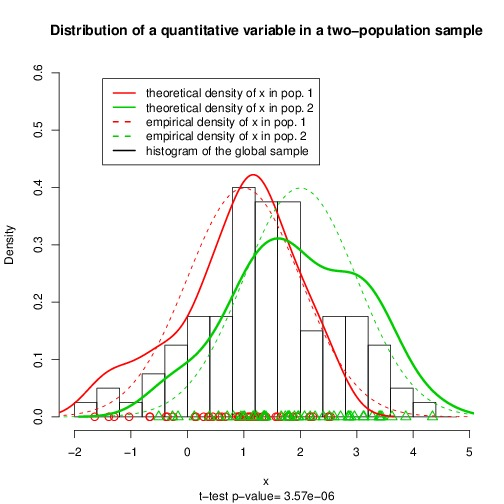
\includegraphics[height=12cm,width=17cm]{../inst/images/power.jpeg}
\caption{Synthetic example of a variable measured in two popualtions with mean equal to 1 and 2 respectively and a common unit variance. 
The global histogram (black) seems unimodal and does not suggest the presence of two populations, the numerical values 
from the two population overlap substantially. Any algorithm aimed at clustering the individuals 
would be subject to a large error rate. However, the p-value of a classical t-test is highly significant.}\label{fig:power}
\end{figure}

\subsection[Ghost clusters]{``Ghost'' clusters}\index{ghost clusters}
{\sc Geneland} outputs include an estimate $\hat{K}$ of the number of clusters present in the sample  
and a map of the geographical locations of these clusters.
It might happen that $\hat{K}$ is larger than the number of clusters observed on this map. The non-observed clusters 
where referred to as ``ghost'' clusters by \cite{Guillot05a}. 
The first version of {\sc Geneland}  \cite{Guillot05a,Guillot05c} was prone to this issue which was mostly due 
to a lack of MCMC mixing corrected in \cite{Guillot08a}. 
This phenomenon can still occur in some instances. 
Imagine for example a set of three individuals for which inference is carried out with an MCMC run of three iterations. 
Denoting $p^t_{i=1,2,3}$ the simulated cluster membership of individual $i$ at iteration $t$ and assuming that 
the chain simulated is $p^1=(2,1,1)$,  $p^2=(1,2,1)$ and  $p^3=(1,1,2)$. The number of clusters simulated along the chain 
is equal to 2 along the whole run. So will be the estimated $K$. However, the three individuals will be assigned 
to cluster 1.
%% The actual estimated cluster memberships will depend on the values of cluster-specific parameters simulated along the chain, which relates 
%% to the so-called label switching issue. 
For data complying well with the modelling assumtptions of {\sc Geneland}, 
and after  relabelling  the simulated cluster memberships\footnote{as explained in \cite{Guillot08a} and performed in {\sc Geneland} 
since version 3.0.0}, such inconsistency on the estimated $K$ was extremely rare.
Occurence of this issue might be an indication of departure of the data from modelling assumptions.

\subsection{Non recombining DNA sequences}\index{sequence data}
DNA sequence data can be analyzed with {\sc Geneland} provided they are stored in the proper format 
(the bases have to be recoded as  $\{1,2,3,4\}$, see section \ref{sec:data_format}). 
Computerwise, analyzing {\em non recombining} DNA sequences does not bring up any difficulty. From a statistical/genetic point of view, 
the meaning and potential outcome of this kind of analyis is less straighforward. {\sc Geneland} assumes linkage equilibirum, an assumption violated in absence of recombination. 
One may expect in some instances that the inferred clusters mirror the spatial location of the main haplogroups. 
This has not been assessed theoretically or empirically as of today. 

\clearpage

\section{Algorithm}\label{sec:algo}

\subsection{Simulation based inference [TODO] }

\subsubsection{Special aspects}
$K_{\mbox{\footnotesize init}}$ set to $K_{\max}$ during the first iterations

\subsection{Post-processing MCMC outputs [TODO] }

\subsubsection{Estimating $K$}

\subsubsection{Dealing with label switching} 

\subsubsection{Computing posterior probability of cluster memberships}


\subsection{F statistics [TODO] }

\begin{itemize}
\item Estimation according to \citet{Weir84}
\item Missing data allowed. Induce a small bias in the estimation of $\Fst$ and a somehow larger bias in the estimation of $\Fis$ .
\item Not implemented for haploid data
\end{itemize}

%%%%%%%%%%%%%%%%%%%%%%%%
\section{Description of MCMC output files }

\subsection{Files produced by MCMC simulations}

Note that some of those files are not created by default. See on-line help for detail.

\subsubsection{\texttt{parameters.txt}}
List of characteristics of the dataset and all arguments passed to function {\it MCMC} (via the GUI or directly).

\subsubsection{\texttt{populations.numbers.txt}}
Simulated values of number of populations $K$.

\subsubsection{\texttt{nuclei.numbers.txt}}
Simulated values of number of Voronoi cell $m$ coding for cluster membership. 
(Set to $n$ under the non-spatial option).


\subsubsection{\texttt{coord.nuclei.txt}}
Simulated coordinates of the nuclei of Voronoi cells in the tessellation uses to parameterise  cluster membership. 
(Set to the coordinates of sampled individuals under the non-spatial option).

\subsubsection{\texttt{color.nuclei.txt}}
Simulated cluster membership of  Voronoi cells. It is coded as an integer and displayed as a color. 


\subsubsection{\texttt{ancestral.frequencies.txt}}
Simulated allele frequencies of ancestral cluster in the correlated allele frequencies model. 

\subsubsection{\texttt{drifts.txt}}
Simulated drift parameter (or  $\Fst$) in the correlated allele frequencies model. 


\subsubsection{\texttt{frequencies.txt}}
Simulated allele frequencies of present time clusters in the correlated allele frequencies model. 


\subsubsection{\texttt{hidden.coord.txt}}
Estimated "true coordinates" if some uncertainty on coordinates is assumed.

\subsubsection{\texttt{log.likelihood.txt}}
Log-likelihood along MCMC simulation.


\subsubsection{\texttt{log.posterior.density.txt}}
Log of posterior density of simulated parameters along MCMC simulation.

\subsection{Files produced when post-processing MCMC simulations}

\subsubsection{\texttt{postprocess.parameters.txt}}
List of all arguments passed to function {\it PostProcessChain} (via the GUI or directly).

\subsubsection{\texttt{proba.pop.membership.txt}}
Posterior probability of cluster membership for pixels of a discretization of the domain.

\subsubsection{\texttt{proba.pop.membership.indiv.txt }}\label{sec:proba.pop.membership.indiv.txt}
Posterior probability of cluster membership for sampled individuals.


\subsubsection{\texttt{modal.pop.txt }}
Estimated cluster membership for pixels of a discretization of the domain.

\subsubsection{\texttt{modal.pop.indiv.txt }}
Estimated cluster membership for sampled individuals.




\subsubsection{\texttt{perm.txt  }}
Permutation of cluster labels allowing to get rid of the label switching issue.




\newpage
\nocite{Guillot05a,Guillot05c,Coulon06,Fontaine07,Guillot08b,Hannelius08,Guillot09c,Guillot09e,Guillot09g,
Guillot09i,Guillot10b,Guillot11b,Guillot12a}

%\bibliography{/media/SSD_Gilles/biogillesg/com/biblio/biblio,/media/SSD_Gilles/biogillesg/com/biblio/gilles}
\bibliography{../inst/biblio,../inst/gilles}

%\include{./Geneland-Doc.bbl}  

\printindex






\end{document}
